\section{Riprogettazione}
Partendo dai problemi di usabilità identificati nella fase di valutazione euristica, si è proceduto alla riprogettazione dell'interfaccia di BrainBox. In primo luogo, sono stati redatti degli scenari d'uso che hanno permesso di mettere a fuoco le criticità più impattanti dal punto di vista dell'utente: simulando situazioni concrete di utilizzo, è stato più semplice individuare i punti in cui l'interfaccia originale risultava carente o confusionaria e definire le scelte progettuali più rilevanti. Questi scenari vengono riportati nei sottocapitoli dedicati alle 
rispettive sezioni. Per quanto riguarda le scelte di layout, struttura visiva e interazione, ci si è invece appoggiati ai design pattern di Jennifer Tidwell, \textit{"Designing Interfaces — Patterns for Effective Interaction Design"} terza edizione e alle leggi della Gestalt, che hanno fornito un riferimento solido su cui basare e giustificare le decisioni progettuali in modo strutturato.

Prima di entrare nel dettaglio delle singole sezioni, vengono presentati i prototipi realizzati in Figma, le scelte di layout adottate per l'intera interfaccia e la palette colori, elementi trasversali che hanno guidato la coerenza visiva dell'intero progetto.

L'attenzione si è concentrata in particolare sulle sezioni principali 
dell'applicazione, \textit{Appunti}, \textit{Esami}, \textit{Community} e gli strumenti AI, che presentavano le criticità più significative e su cui è stato necessario intervenire in modo più profondo, ripensando non solo aspetti di dettaglio ma in alcuni casi la struttura stessa delle sezioni. Sono state comunque riviste anche \textit{Homepage}, \textit{Registrazione e Login} e \textit{Dashboard}, con interventi più mirati sui problemi riscontrati. Per ciascuna sezione vengono descritti i pattern applicati, le modifiche apportate e i problemi di usabilità 
risolti; nei casi in cui un problema non sia stato affrontato o sia stato rivalutato, viene fornita una spiegazione esplicita della scelta.

\paragraph{Prototipi}
Prima di procedere con l'implementazione, le principali scelte progettuali sono 
state tradotte in prototipi realizzati con Figma. L'obiettivo non era definire 
ogni dettaglio visivo, ma fissare le idee progettuali più rilevanti, struttura 
delle pagine, organizzazione dei contenuti e collocazione degli elementi 
principali, in modo da avere un riferimento condiviso durante lo sviluppo. 
Di seguito vengono presentati i prototipi che rispecchiano più fedelmente 
il risultato implementato; altri mockup realizzati durante la fase progettuale 
non vengono riportati in quanto hanno subito modifiche durante lo sviluppo, 
dovute sia a rivalutazioni delle scelte di usabilità sia a vincoli tecnici 
emersi in fase di implementazione.

\begin{figure}[H]
    \centering
    \fbox{\includesvg[width=0.7\textwidth]{./figures/mockup/Pagina Registrazione Step 1}}
    \caption{Mockup della modale}
    \label{fig:mockup_registrazione}
\end{figure}

Il primo prototipo di Figura \ref{fig:mockup_registrazione} illustra la struttura della modale utilizzata per i form multi-step, di cui la registrazione rappresenta un esempio. Questa struttura è stata mantenuta coerente in tutte le modali presenti nell'applicazione, garantendo all'utente un'esperienza uniforme indipendentemente dall'operazione che sta compiendo. L'idea progettuale era quella di offrire un form pulito e focalizzato, in cui l'utente sa sempre a che punto si trova grazie all'indicatore degli step, può tornare indietro in qualsiasi momento senza perdere i dati già inseriti e, prima di confermare, ha la possibilità di rivedere un riepilogo 
di tutto ciò che ha compilato.

\begin{figure}[H]
    \centering
    \fbox{\includesvg[width=0.7\textwidth]{./figures/mockup/Dashboard}}
    \caption{Mockup dashboard}
    \label{fig:mockup_dashboard}
\end{figure}

\begin{figure}[H]
     \centering
     \begin{subfigure}[b]{0.3\textwidth}
         \centering
         \fbox{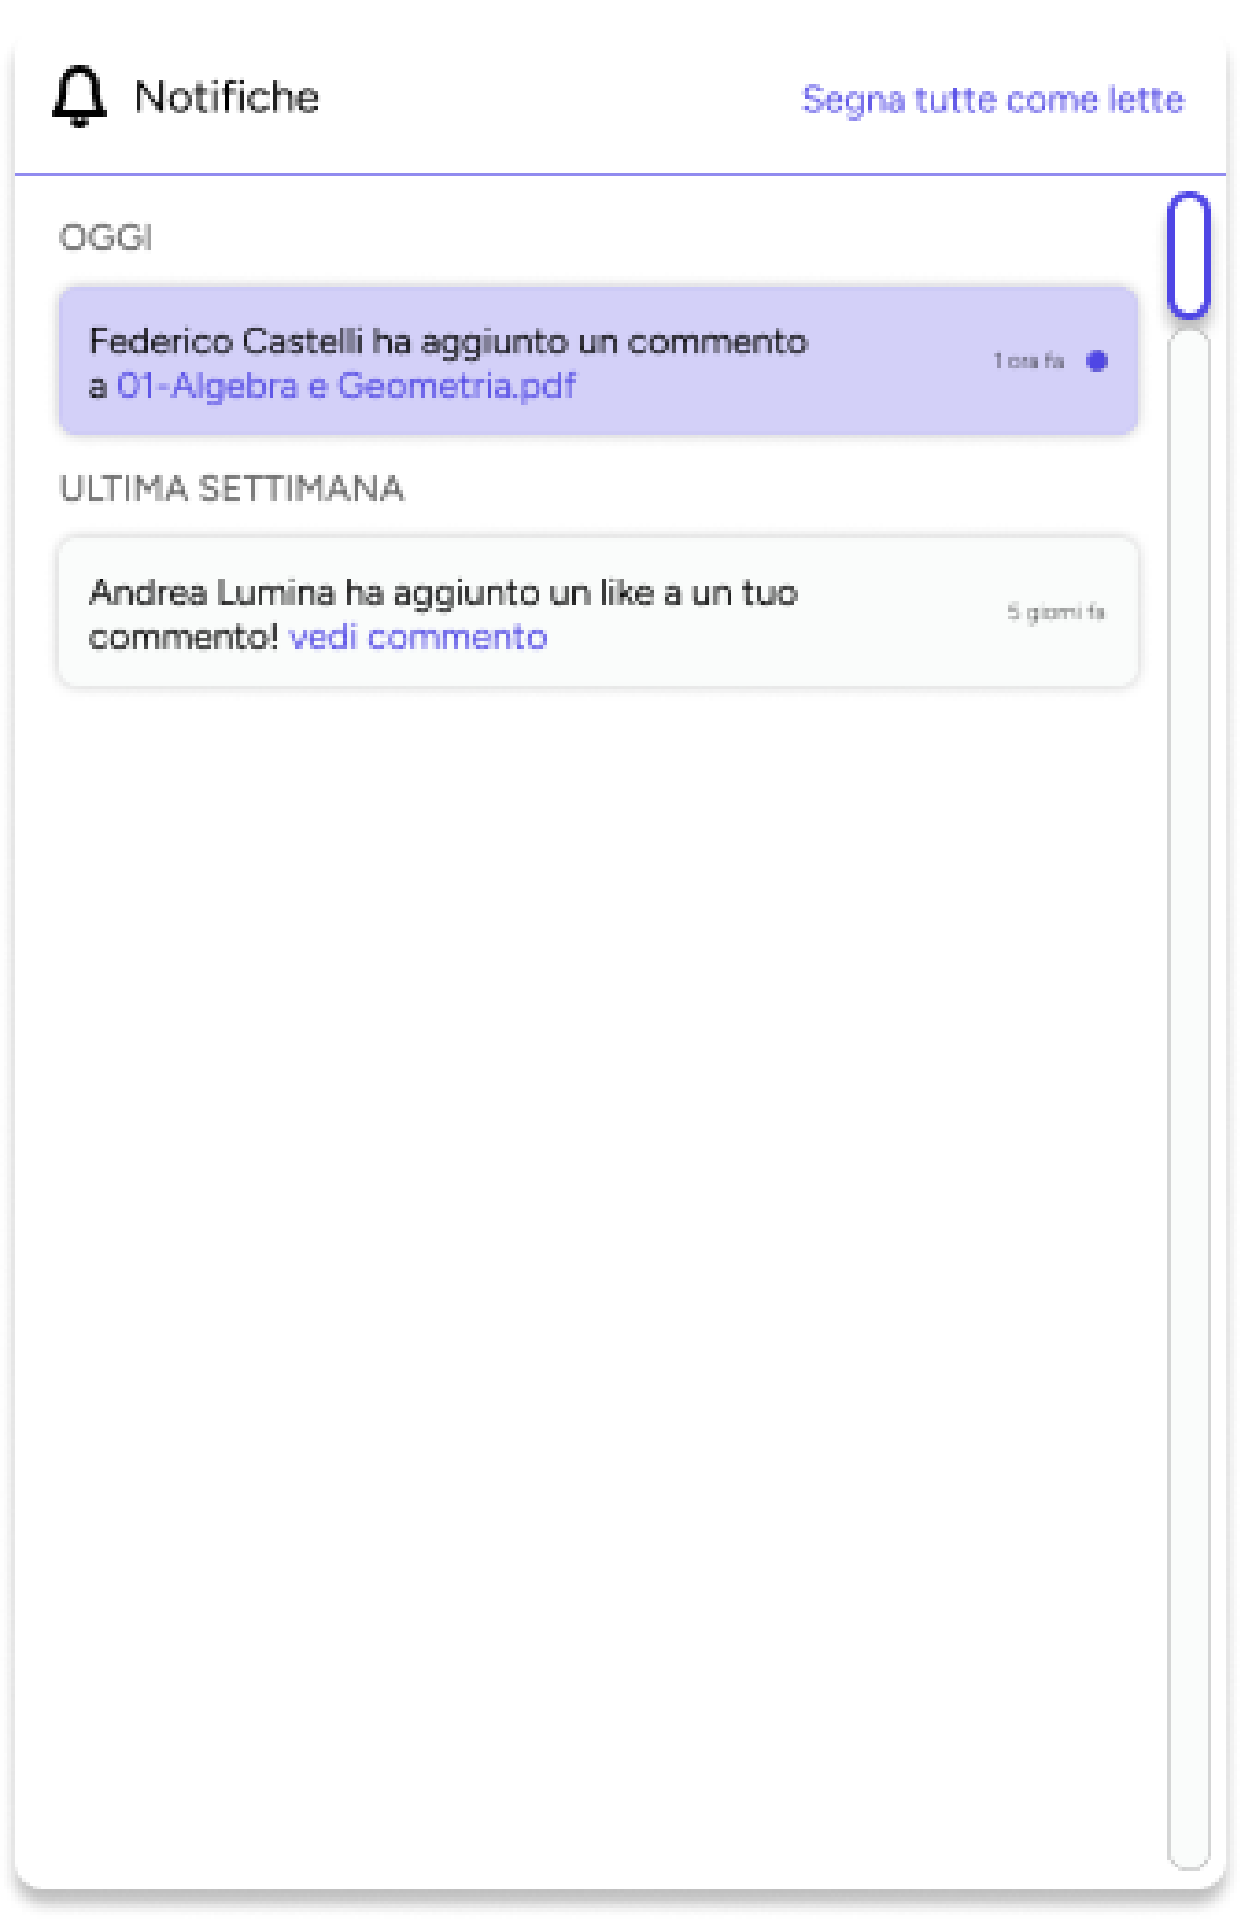
\includegraphics[width=\textwidth]{./figures/mockup/menu-tendina-notifiche}}
         \caption{Menu notifiche}
         \label{fig:notifiche}
     \end{subfigure}
     \qquad
     \begin{subfigure}[b]{0.3\textwidth}
         \centering
         \fbox{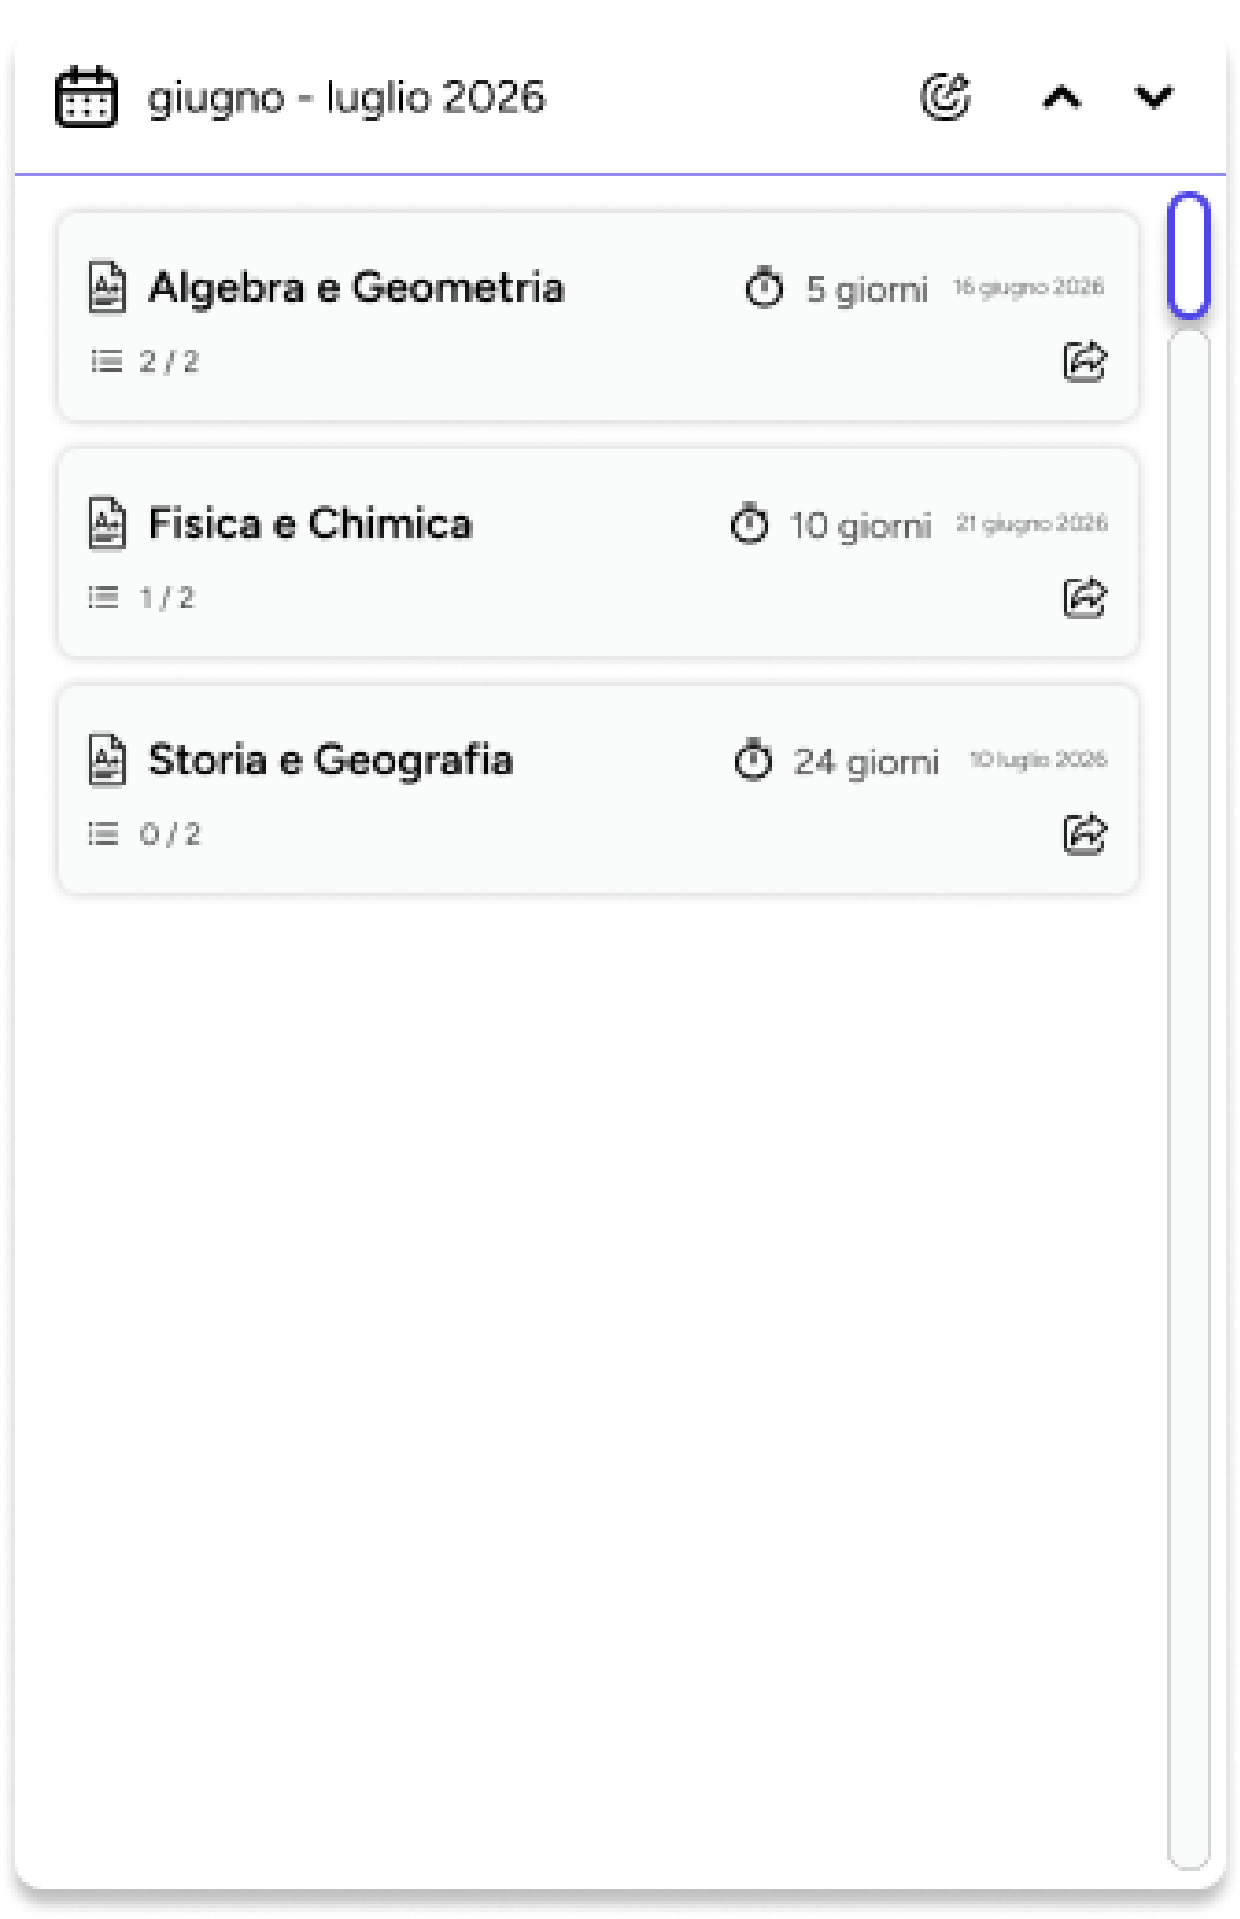
\includegraphics[width=\textwidth]{./figures/mockup/menu-tendina-calendario}}
         \caption{Menu calendario}
         \label{fig:calendario}
     \end{subfigure}
     
     \caption{}
     \label{fig:mockup_menu}
\end{figure}

Il secondo prototipo di Figura \ref{fig:mockup_dashboard} mostra la \textit{Dashboard} riprogettata, che permette di apprezzare alcune delle scelte progettuali più rilevanti dell'intera applicazione. Il pannello di navigazione sinistro è stato completamente rivisto: i nomi delle sezioni sono stati semplificati e resi immediatamente comprensibili, e le funzionalità AI sono state accorpate all'interno di \textit{Appunti}, dove risulta più logico trovarle in quanto i file generati vengono salvati e gestiti insieme agli altri materiali di studio. La \textit{Dashboard} stessa è stata ridisegnata nella suddivisione in blocchi, offrendo una panoramica più chiara e interattiva dell'attività dell'utente e fungendo da anteprima delle principali sezioni dell'applicazione.

La Figura \ref{fig:notifiche} e la Figura \ref{fig:calendario} successive mostrano invece il menu delle notifiche e il menu del calendario, entrambi progettati da zero in quanto assenti nella versione originale. Il calendario in particolare è stato spostato nella navbar, rendendolo accessibile da qualsiasi sezione dell'applicazione senza dover navigare altrove, così da permettere all'utente di consultare le scadenze degli esami in qualsiasi momento.

\begin{figure}[H]
    \centering
    \fbox{\includesvg[width=0.7\textwidth]{./figures/mockup/Appunti - apri file}}
    \caption{Mockup visualizzazione appunti}
    \label{fig:mockup_appunti}
\end{figure}

L'ultimo prototipo di Figura \ref{fig:mockup_appunti} illustra la pagina di visualizzazione di un documento. La scelta progettuale è stata quella di mantenere la struttura generale già presente nella versione originale, intervenendo principalmente sulla chiarezza del pannello laterale destro. In particolare, le informazioni sono state organizzate in due blocchi distinti e visivamente separati (oltre ad un blocco, aggiunto in fase di implementazione, che specifica il nome utente a cui appartiene il documento): i dettagli del documento nella parte superiore e la sezione commenti in quella inferiore, poiché nella versione precedente la mancanza di una separazione netta rendeva il pannello confusionario.

\paragraph{Layout}
La struttura utilizzata nelle pagine interne riprende quella della versione originale del sito. Si tratta di una sorta di column grid, composta da una sidebar fissa a sinistra che contiene la navigazione principale, e da un'area di contenuto a destra che occupa la parte restante dello schermo. Questa organizzazione permette all'utente di sapere sempre dove si trova all'interno dell'applicazione, mantenendo la navigazione sempre visibile e accessibile. La separazione tra le due aree crea inoltre un raggruppamento visivo chiaro, che aiuta l'utente a distinguere immediatamente gli elementi di navigazione dal contenuto della pagina.

Durante la riprogettazione dell'interfaccia si è tenuto conto delle \textit{leggi della Gestalt}, principi visivi che guidano il modo in cui l'utente percepisce e interpreta ciò che vede sullo schermo. Nella versione originale del sito alcune di queste leggi non erano sempre rispettate, e questo è stato uno degli aspetti su cui si è cercato di intervenire. La \textit{legge di prossimità}, ad esempio, suggerisce che elementi vicini tra loro vengono percepiti come appartenenti allo stesso gruppo: nell'interfaccia riprogettata questo si vede nella sidebar, dove le voci di navigazione sono raggruppate vicine tra loro, oppure nei form, dove ogni label è posizionata subito sopra al campo a cui si riferisce. La \textit{legge di chiusura} è invece alla base dell'uso delle card, che grazie al bordo arrotondato e allo sfondo bianco creano un contenitore visivo ben definito, rendendo immediato capire quali informazioni fanno parte dello stesso blocco. La \textit{legge di similarità} si applica al modo in cui tutti i bottoni principali condividono la stessa forma e lo stesso colore azzurro, così come tutte le voci della sidebar hanno la stessa dimensione e lo stesso stile, aiutando l'utente a riconoscere elementi con la stessa funzione. Infine la \textit{legge del contrasto} è usata per far emergere le azioni principali: il bottone azzurro su sfondo bianco cattura subito l'attenzione, guidando l'utente verso l'azione che ci si aspetta compia.

\paragraph{Palette colori}
La palette adottata per l'interfaccia di BrainBox è composta da quattro colori principali: il bianco, il grigio chiaro, l'azzurro e il nero. La scelta di questi colori segue la regola 60-30-10 di Michal Malewicz, che indica come ripartire i colori in un'interfaccia per ottenere un risultato visivamente bilanciato. Il 60\% dello spazio è occupato dal colore dominante, in questo caso bianco e grigio chiaro insieme, che copre gli elementi più grandi come lo sfondo delle pagine, le card e la sidebar, dando all'interfaccia un aspetto pulito e non pesante. Il 30\% è invece riservato all'azzurro, che è il colore che caratterizza l'interfaccia e compare su tutti gli elementi con cui l'utente interagisce: bottoni, link, bordi dei campi di testo e voci di navigazione attive. Il nero chiude con il 10\%, usato solo per testo e icone: poca superficie, ma con un contrasto molto alto che rende tutto facilmente leggibile. La scelta di usare solo quattro colori, senza aggiungere sfumature o colori extra, è stata fatta per tenere l'interfaccia semplice e coerente. Fanno eccezione il verde e il rosso, usati in modo molto limitato per i badge di stato, come ad esempio per indicare se un appunto è pubblico o se un esame è scaduto. Il contrasto tra i colori è stato verificato con la formula di luminanza percepita del W3C, che ha confermato che in tutti i casi il testo risulta leggibile sullo sfondo corrispondente.

\begin{figure}[H]
    \centering
    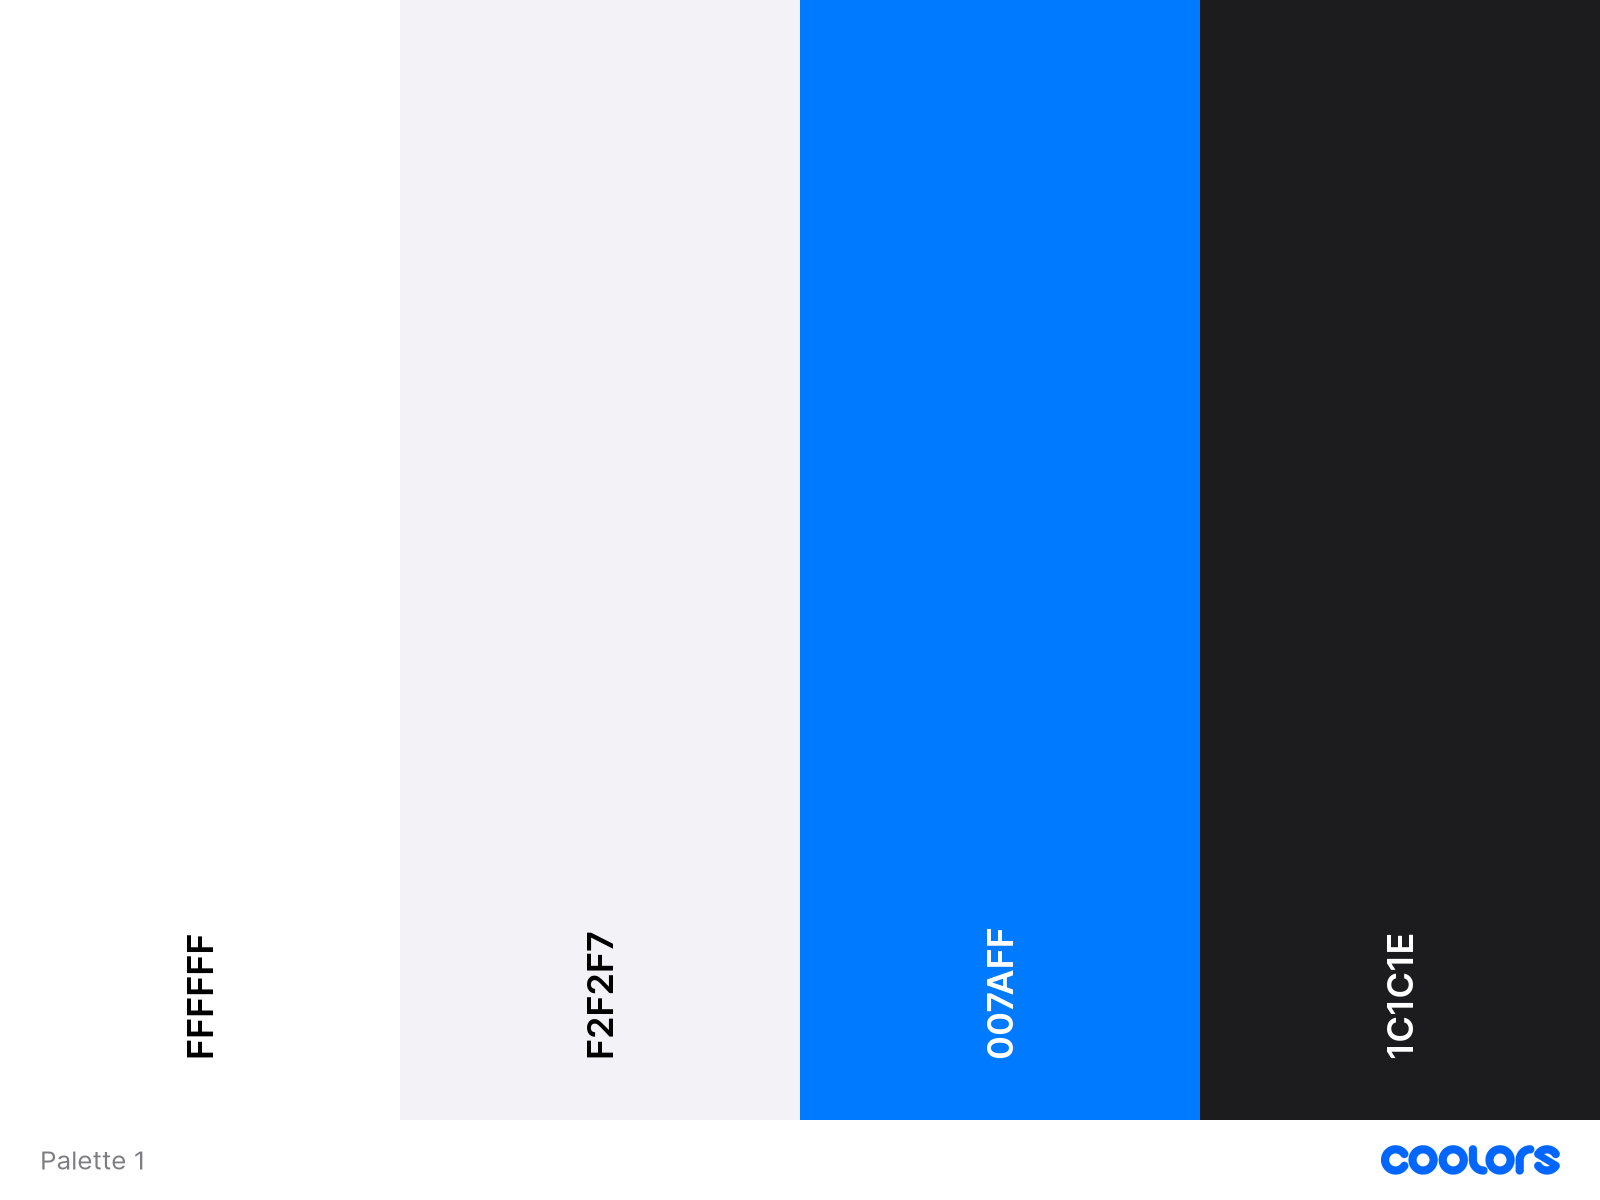
\includegraphics[width=0.8\textwidth]{figures/fig-riprogettazione-fisica/palette1.png}
    \caption{Palette}
    \label{fig:palette}
\end{figure}

\subsection{Homepage}
La homepage mantiene la struttura originale: suddivisa in header, sezione di benvenuto, funzionalità, prezzi e footer. L'obiettivo principale è rimasto quello di presentare la piattaforma ai nuovi utenti e invitarli a registrarsi. In questa fase si è scelto di non stravolgere l'impostazione iniziale, dato che la homepage non è emersa come la sezione più critica del sito e non presentava tanti problemi di usabilità. L'intervento si è quindi limitato alla risoluzione dei problemi riscontrati, senza spostare il focus dalle aree del sistema che richiedevano maggiore attenzione.

\paragraph{Design pattern applicati}

\begin{itemize}
    \item \textbf{Sign-In Tools} (Tidwell): Il pattern prevede di posizionare nella parte superiore destra dell'interfaccia i controlli di accesso, come i pulsanti di login e registrazione, in quanto è la posizione convenzionale in cui gli utenti si aspettano di trovarli. Nella versione precedente il pulsante di accesso "Accedi" aveva un aspetto meno evidente rispetto a "Inizia Subito", risultando quasi non cliccabile, e i due pulsanti non comunicavano chiaramente la distinzione tra accesso e registrazione. Nella versione riprogettata entrambi i pulsanti sono stati uniformati graficamente e rinominati in "Accedi" e "Registrati", rendendone immediatamente chiaro il ruolo e la differenza.

    Problemi di usabilità risolti:
    \begin{itemize}
        \item P1 (Il pulsante "Inizia Subito" dovrebbe essere "Registrati" per coerenza con "Accedi"): Il pulsante è stato rinominato \textit{"Registrati"}.
        \item P81 (Il pulsante "Accedi" è meno evidente e può sembrare non cliccabile): I due pulsanti sono stati uniformati graficamente e accorpati in alto a destra.
    \end{itemize}

\end{itemize}

\paragraph{Altre modifiche}
Sono state inoltre apportate diverse correzioni mirate a migliorare la coerenza e l'usabilità dell'interfaccia nella homepage. In particolare, è stata eliminata la duplicazione del pulsante \textit{Inizia Subito}, mantenendo un'unica call-to-action principale per evitare ambiguità. La sezione dei piani di abbonamento è stata resa più visibile e uniforme, seguendo l'idea dei mockup, migliorando il contrasto e rimuovendo lo sfondo trasparente per una maggiore leggibilità. Tutti i pulsanti associati ai piani sono stati resi coerenti sia nel testo sia nel comportamento: le etichette sono state uniformate in \textit{Registrati} e ogni bottone risulta ora correttamente cliccabile. Infine, nel footer sono stati rimossi i collegamenti non funzionanti sotto le sezioni \textit{Azienda} e \textit{Legale}, lasciando solo i link attivi a \textit{Funzionalità} e \textit{Prezzi}, che indirizzano correttamente alle rispettive sezioni della pagina. \\

Problemi di usabilità risolti:
\begin{itemize}
    \item P2 (Duplicazione del pulsante "Inizia Subito"): È stato rimosso il pulsante centrale, mantenendo un'unica call-to-action in alto a destra.
    \item P4 (Le sezioni dei piani di abbonamento non sono ben visibili): Le card sono state uniformate e rese più evidenti, eliminando lo sfondo trasparente.
    \item P5 (Il pulsante "Get Started" nei piani non è cliccabile): Tutti i pulsanti sono stati resi cliccabili e rinominati \textit{Inizia ora}.
    \item P6 (Il piano "Standard" ha un pulsante non cliccabile): Il pulsante è ora attivo e coerente con gli altri (\textit{Inizia ora}).
    \item P7 (Testo incoerente del pulsante "Inizia Subito, Gratis"): Il testo è stato uniformato a \textit{Registrati}.
    \item P8 (Link non funzionanti nel footer): Rimossi i link non attivi e mantenuti solo quelli funzionanti.
\end{itemize}
\subsubsection{Registrazione e Login}

\begin{scenario}{Scenario: Registrazione e Login}
  Ho deciso di iscrivermi a BrainBox per gestire meglio il mio studio.
  Una volta aperta la pagina di registrazione, noto subito che \textbf{non avendo un indicatore di avanzamento, non so quanti
  passaggi manchino} per completare il profilo.

  Inizio inserendo i dati personali e scelgo una password. In questa fase, mi
  accorgo che \textbf{non posso visualizzare i caratteri digitati} e quindi non posso verificare se ho scritto correttamente la password. Infatti, dopo aver confermato, compare un \textbf{messaggio d'errore in lingua inglese}, che mi risulta fuori luogo
  rispetto al resto dell'interfaccia in italiano.

  Superata questa fase, passo ai dettagli accademici. Aprendo il menu a tendina
  per l'ateneo, noto che \textbf{la voce} \textit{«Seleziona la tua università»} \textbf{è
  elencata come se fosse un'opzione selezionabile}, e lo stesso accade per i
  campi \textit{«Dipartimento»} e \textit{«Ciclo di studi»}.

  Qualche giorno dopo, provo a effettuare il Login. Anche in questo caso, digito con cautela la password dato che \textbf{non ho la possibilità di visualizzarla}. Sbaglio un carattere e appare nuovamente un \textbf{avviso in inglese}.

  Scopro inoltre che, sia nella fase di Registrazione sia nella fase di Login, \textbf{se volessi tornare alla Homepage o al passaggio precedente, per correggere un dato o annullare l'operazione, non c'è alcuna possibilità} se non cliccando dal tasto \textit{«Torna indietro»} del browser.
\end{scenario}

\paragraph{Design pattern applicati}
\begin{itemize}
  \item \textbf{Wizard + Modal Panel + Progress Indicator} (Tidwell): Il flusso di registrazione era già strutturato parzialmente come un wizard, un componente che guida l'utente passo dopo passo in un ordine prestabilito, indicato per task lunghi o complessi che l'utente affronta raramente, come la creazione di un profilo. L'intero wizard è presentato come un pannello sovrapposto all'interfaccia, concentrando l'attenzione dell'utente esclusivamente sul processo di registrazione senza distrazioni. Tramite questo pattern è stata aggiunta la possibilità di navigare liberamente tra gli step con un pulsante \textit{Indietro}, senza perdere i dati già inseriti. È inoltre possibile abbandonare l'operazione in qualsiasi momento tramite \textit{due link} (uno che porta alla pagina di Login/Registrazione e un altro che porta alla Homepage). Per quanto riguarda gli step, è stato seguito il pattern Progress Indicator, che prevede di mostrare su ogni pagina del wizard una mappa degli step con un indicatore, così l'utente sa esattamente dove si trova e quanto manca alla fine.

    Problemi di usabilità risolti:
    \begin{itemize}
      \item P10 (Non è possibile tornare alla homepage): è stato aggiunto un link, nella parte inferiore dei form di Registrazione e Login, che porta direttamente alla homepage.
      \item P54 (Nessun indicatore di progresso nel form di Registrazione): sono stati inseriti degli step per indicare all'utente a che punto si trova durante il processo di Registrazione.
    \end{itemize}

  \item \textbf{Password Strength Meter} (Tidwell): E' stato applicato questo pattern per permettere all'utente di avere un'idea chiara della robustezza della password che sta inserendo ed evitare di fargli fare molti tentativi prima di inserirla nel formato consentito. Inoltre, per supportare l'utente nella scelta e nell'inserimento della password, è stata adottata la soluzione indicata all'interno di questo pattern: rendere visibile un \textit{toggle} che consente di visualizzare i caratteri digitati. Come indicato dal pattern, il campo password non dovrebbe mostrare i caratteri di default, ma offrire all'utente la possibilità di farlo tramite un'apposita opzione. (Figura \ref{fig:registrazione_2})

    Problemi di usabilità risolti:
    \begin{itemize}
      \item P18 (Non è possibile visualizzare la password inserita): è stato aggiunto un toggle (occhiolino) per mostrare/nascondere la password inserita.
    \end{itemize}

  \item \textbf{Error Messages} (Tidwell): Il pattern prevede che i messaggi di errore siano posizionati direttamente nel form, vicino al campo che li ha generati, e scritti in linguaggio comprensibile per l'utente. Nel caso di BrainBox, i messaggi di errore apparivano in lingua inglese in un'interfaccia in italiano. La soluzione adottata è stata quella di tradurre i messaggi in italiano, rendendoli coerenti con il resto dell'interfaccia.

    Problemi di usabilità risolti:
    \begin{itemize}
      \item P9 (Il testo nei form di login e registrazione è in inglese): è stato tradotto il testo, compresi i messaggi di errore.
    \end{itemize}
\end{itemize}

\begin{figure}[H]
    \centering
    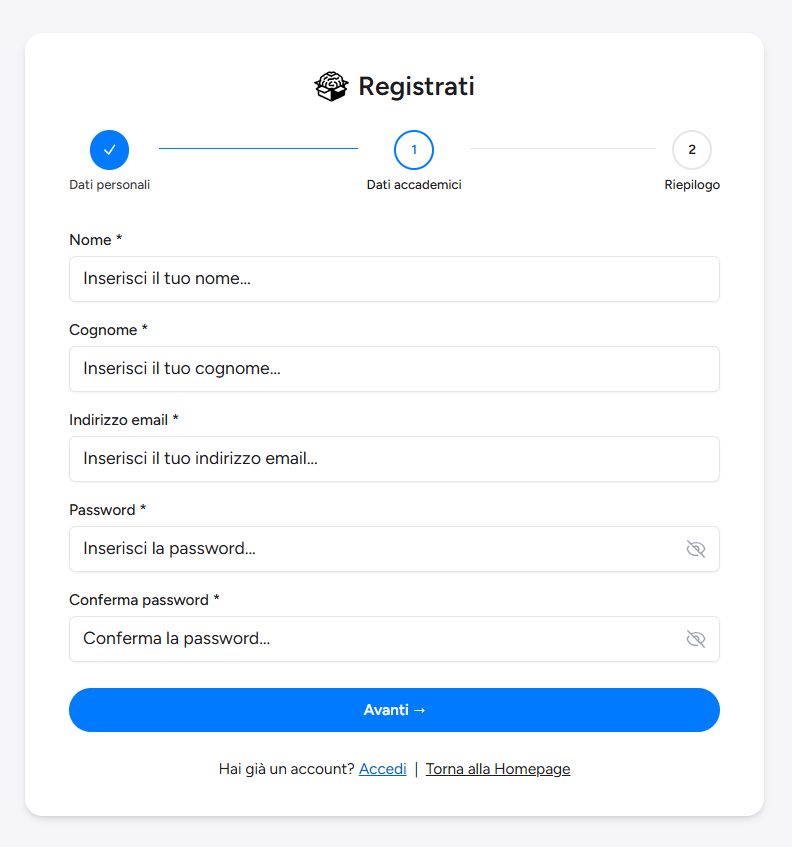
\includegraphics[width=0.6\textwidth]{figures/fig-riprogettazione-fisica/registrazione-login/registrazione_1.png}
    \caption{Step 1 Registrazione}
    \label{fig:registrazione_1}
\end{figure}

\begin{figure}[H]
    \centering
    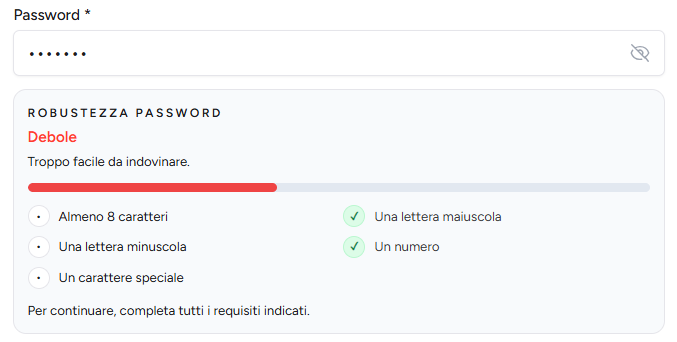
\includegraphics[width=0.6\textwidth]{figures/fig-riprogettazione-fisica/registrazione-login/registrazione_2.png}
    \caption{Controllo robustezza password}
    \label{fig:registrazione_2}
\end{figure}

\begin{figure}[H]
    \centering
    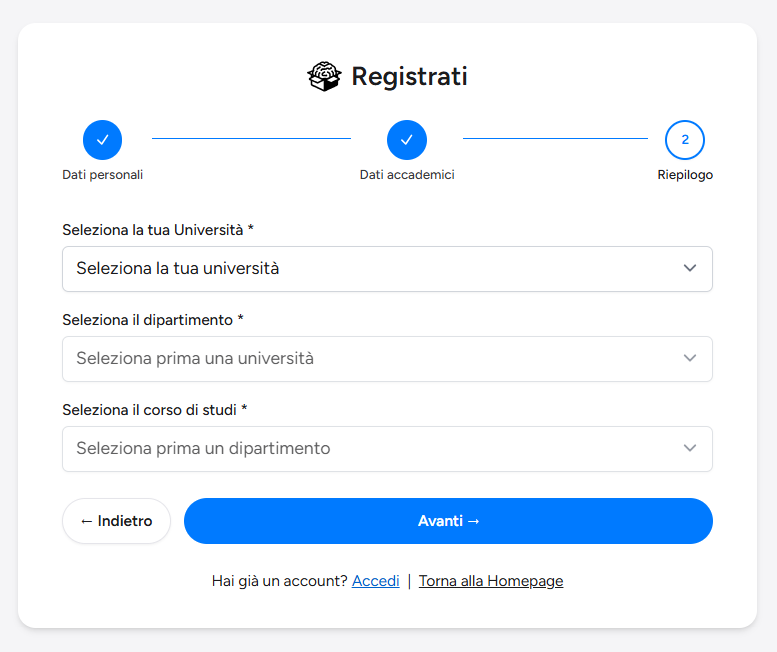
\includegraphics[width=0.6\textwidth]{figures/fig-riprogettazione-fisica/registrazione-login/registrazione_3.png}
    \caption{Step 2 Registrazione}
    \label{fig:registrazione_3}
\end{figure}

\begin{figure}[H]
    \centering
    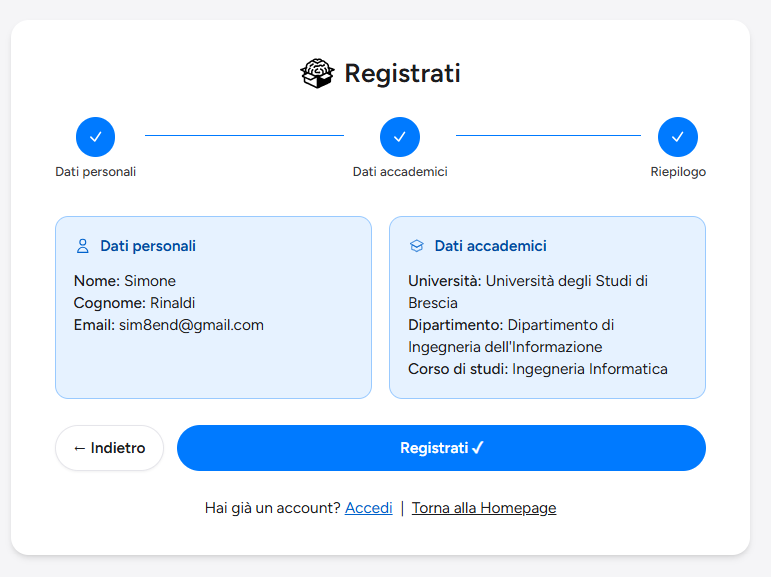
\includegraphics[width=0.6\textwidth]{figures/fig-riprogettazione-fisica/registrazione-login/registrazione_4.png}
    \caption{Step 3 Registrazione}
    \label{fig:registrazione_4}
\end{figure}

\begin{figure}[H]
    \centering
    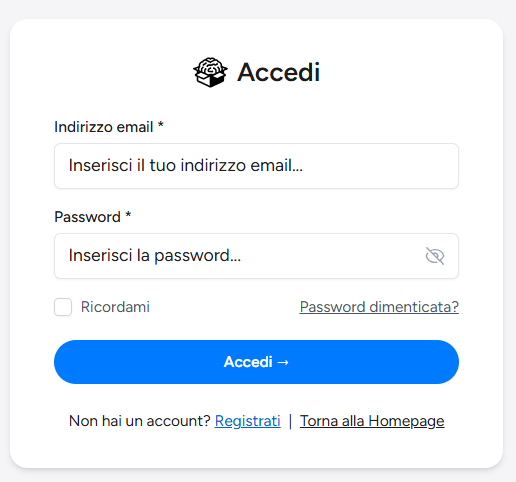
\includegraphics[width=0.6\textwidth]{figures/fig-riprogettazione-fisica/registrazione-login/accedi_1.png}
    \caption{Modale Accedi}
    \label{fig:accedi_1}
\end{figure}
\subsection{Navbar e sidebar}
Una volta effettuato l'accesso, l'utente si trovava davanti a una schermata principale di lavoro composta da una navbar, tramite la quale era possibile accedere alle notifiche, cambiare tema e gestire le impostazioni del profilo, e da una sidebar sulla sinistra che elencava le sezioni principali dell'applicazione: \textit{MyAcademia Dashboard}, \textit{I Miei Appunti}, \textit{Esplora Appunti}, \textit{Sbobinatore AI}, \textit{Audio Note AI} e \textit{StudyFlow AI}. Questa configurazione risultava difficile da interpretare per due motivi principali: i nomi delle sezioni non comunicavano chiaramente la loro funzionalità e alcuni erano in inglese, in contrasto con il resto dell'interfaccia in italiano. Inoltre le notifiche non erano funzionanti. Per tali ragioni si è deciso di riprogettare la navbar e la sidebar, mantenendo invariata la struttura generale e intervenendo principalmente sulla chiarezza e la coerenza linguistica dei contenuti.

\paragraph{Design pattern applicati}
\begin{itemize}
  \item \textbf{Sign-In Tools} (Tidwell): Il pattern prevede di posizionare nella parte superiore destra dell'interfaccia gli strumenti trasversali legati all'esperienza dell'utente autenticato, accessibili da qualunque schermata indipendentemente dalla sezione aperta. Alcune voci possono essere esposte direttamente come icone nella navbar, mentre altre possono essere nascoste in un menu a tendina accessibile dal nome utente o dall'avatar. Nella versione riprogettata di BrainBox, la navbar è stata arricchita rendendo funzionanti le notifiche e aggiungendo un accesso diretto al calendario, entrambi espandibili a tendina, mantenendo il nome utente con menu a tendina per le impostazioni del profilo e il logout.

    Problemi di usabilità risolti:
    \begin{itemize}
      \item P12 (Notifiche non funzionanti): Sono state attivate le notifiche, per permettere all'utente di ricevere avvisi riguardanti scadenze e attività della community.
      \item P88 (Calendario non funzionante): E' stato reso funzionante il calendario e collocato nella navbar, a differenza della versione precedente nella quale era visibile solo accedendo alla sezione \textit{Exam Details}.
    \end{itemize} 
\end{itemize}

\paragraph{Altre modifiche} 
Il testo della sidebar e della navbar è stato tradotto in italiano per garantire coerenza linguistica con il resto dell'interfaccia. Le sezioni sono state rinominate con etichette più immediate e comprensibili: \textit{Dashboard}, \textit{Appunti}, \textit{Esami} e \textit{Community}. Le due sezioni dedicate agli strumenti AI, sbobinatore e generatore di audio note, sono state accorpate all'interno di \textit{Appunti}: nella versione precedente, le trascrizioni e le audio note generate venivano salvate nelle rispettive sezioni dedicate, impedendo all'utente di organizzarle insieme agli altri file nelle cartelle di \textit{Appunti}. Centralizzando tutto in un'unica sezione, l'utente può gestire e riorganizzare liberamente l'intero materiale di studio in un solo posto. \\

Problemi di usabilità risolti:
\begin{itemize}
  \item
  \begin{itemize}
      \item P90 (”Your Exams” accessibile tramite ”StudyFlow AI”, collocata in ”Strumenti AI”, il che risulta poco pertinente rispetto alla sua funzione): La sezione per accedere ai propri esami è stata rinominata \textit{Esami} ed è stata rimossa l'etichetta \textit{Strumenti AI} perchè le funzionalità AI sono state accorpate in \textit{Appunti}.
  \end{itemize}
\end{itemize}

\begin{figure}[H]
    \centering
    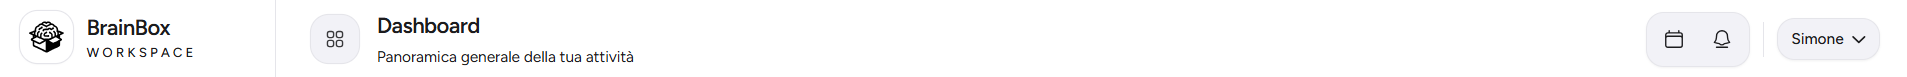
\includegraphics[width=0.8\textwidth]{figures/fig-riprogettazione-fisica/navbar-sidebar/navbar.png}
    \caption{Navbar}
    \label{fig:navbar}
\end{figure}

\begin{figure}[H]
    \centering
    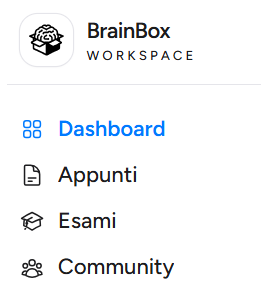
\includegraphics[width=0.3\textwidth]{figures/fig-riprogettazione-fisica/navbar-sidebar/sidebar.png}
    \caption{Sidebar}
    \label{fig:sidebar}
\end{figure}

\begin{figure}[H]
    \centering
    \begin{subfigure}[b]{0.47\textwidth}
        \centering
        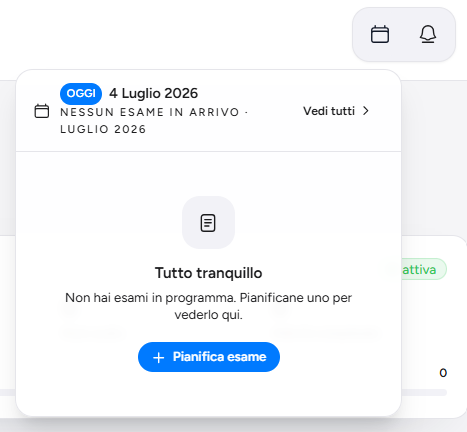
\includegraphics[width=0.8\textwidth]{figures/fig-riprogettazione-fisica/navbar-sidebar/calendario.png}
        \caption{Calendario}
        \label{fig:calendario_navbar}
    \end{subfigure}
    \qquad
    \begin{subfigure}[b]{0.47\textwidth}
        \centering
        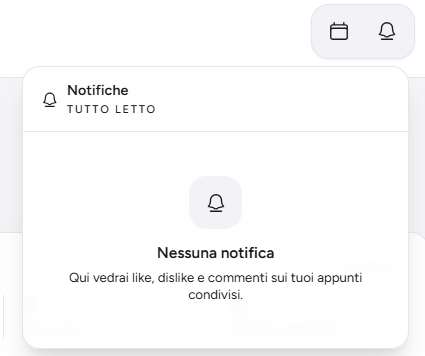
\includegraphics[width=0.8\textwidth]{figures/fig-riprogettazione-fisica/navbar-sidebar/notifiche.png}
        \caption{Notifiche}
        \label{fig:notifiche_navbar}
    \end{subfigure}

    \caption{}
    \label{fig:calendario_notifiche}
\end{figure}

\subsection{Dashboard}

La Dashboard è la prima schermata che l'utente vede dopo l'accesso e funge da pannello di controllo generale dell'esperienza su BrainBox. Nella versione precedente 
presentava statistiche aggregate, una sezione per gli esami in programma e un elenco delle attività recenti, ma con testi in parte in inglese e una struttura visiva poco organizzata. Nella versione riprogettata la Dashboard è stata tradotta interamente in italiano e arricchita: accoglie l'utente con un messaggio di benvenuto personalizzato, mostra una panoramica delle attività della settimana, gli esami imminenti con indicazione dei giorni rimanenti, le attività pianificate per oggi e gli appunti 
caricati di recente, tutti raggiungibili con un link diretto alla sezione corrispondente.

\paragraph{Design pattern applicati}

\begin{itemize}
    \item \textbf{Dashboard} (Tidwell): Il pattern prevede di raccogliere in un'unica 
    pagina i dati e le informazioni più rilevanti per l'utente, aggiornati in tempo reale, in modo che possa ottenere una panoramica immediata della propria situazione senza 
    dover navigare tra le diverse sezioni. Nella versione riprogettata la Dashboard centralizza in un colpo d'occhio lo stato degli appunti, degli esami imminenti, delle 
    attività di oggi e dell'attività settimanale, riducendo il bisogno di spostarsi tra le sezioni per raccogliere queste informazioni.

    \item \textbf{Titled Sections} (Tidwell): Il pattern prevede di suddividere una pagina densa di contenuti in sezioni distinte, ciascuna con un titolo visivamente riconoscibile, per facilitare la scansione e la comprensione immediata della struttura. Nella versione riprogettata la Dashboard è organizzata in blocchi chiaramente separati (\textit{Panoramica}, \textit{Questa settimana}, \textit{Esami}, 
    \textit{Attività di oggi} e \textit{Appunti recenti}) ognuno con titolo e contenuto omogeneo, rendendo immediato per l'utente identificare l'informazione che cerca.

    \item \textbf{One-Window Drilldown} (Tidwell): Il pattern prevede di mostrare una lista di elementi in una schermata e di permettere all'utente di accedere al dettaglio di ciascuno navigando nella sezione corrispondente. Nella Dashboard ogni sezione espone un riepilogo degli elementi più recenti o rilevanti (ultimi appunti, prossimi esami, attività di oggi) accompagnato da un link \textit{"Vedi tutti"} che porta direttamente alla sezione dedicata, evitando di sovraccaricare la Dashboard con informazioni complete.

\end{itemize}

\paragraph{Altre modifiche}
Il testo dell'interfaccia è stato interamente tradotto in italiano. Il pulsante 
\textit{"Passa a BrainBox Pro +"} (P17), presente nella versione precedente senza 
alcuna funzione attiva, è stato rimosso.

Problemi di usabilità risolti:
\begin{itemize}
  \item P11 (Mix italiano/inglese nella dashboard): Tutto il testo è stato tradotto 
  in italiano.
  \item P17 (Il pulsante "Passa a BrainBox Pro +" non è funzionante): Il pulsante è stato rimosso perché non era collegato a una funzione reale. Dato che la riprogettazione non ha riguardato il sistema degli abbonamenti, lasciarlo attivo avrebbe solo confuso l'utente con un comando inutile.
\end{itemize}
\subsection{Appunti}

\begin{scenario}{Scenario: Primo accesso alla pagina I Miei Appunti}
  Accedo alla pagina che dovrebbe chiamarsi \textit{«I Miei Appunti»}, ma la prima cosa che noto è il titolo della sezione (\textit{«Resource Repository»}) che è \textbf{in inglese e non coerente con il link che ho appena cliccato}. Davanti a me compaiono due avvisi che mi segnalano l'assenza
  di cartelle e documenti principali; capisco che è logico, visto che non ho ancora caricato nulla, ma mi sarei aspettato un invito tipo \textit{«Carica qui il tuo primo file»}. Cerco i tasti per iniziare, ma \textbf{non sono dentro la pagina}: devo
  risalire con lo sguardo fino alla barra di navigazione in alto per trovare i pulsanti \textit{«Carica file»} e \textit{«Nuova cartella»}. 

  Procedo comunque a creare la mia prima cartella. Il sistema mi chiede il nome e se voglio renderla pubblica tramite un flag; clicco su \textit{«Crea cartella»} e vedo che l'operazione va a buon fine. Entro nella cartella appena creata, ma mi ritrovo al punto di partenza: compare di nuovo il messaggio che non sono stati trovati documenti e, per creare una sotto-cartella, devo di nuovo andare a cercare il tasto in alto nella navbar. Una volta creata anche la sotto-cartella, \textbf{cerco un tasto} \textit{«Indietro»} \textbf{per risalire il percorso, ma non lo trovo}. Mi accorgo
  però che esiste una traccia del percorso tipo \textit{«Dashboard $>$ I Miei Materiali $>$ Cartella 1»}: clicco lì sopra per muovermi tra i livelli.

  Decido finalmente di caricare un file. Si apre una schermata dove posso trascinare il documento e noto una barra di avanzamento divisa in tre step: \textit{«Upload»}, \textit{«Dettagli»} e \textit{«Fatto»}. Provo a caricare un PDF, ma \textbf{il sistema si blocca e mi restituisce una scritta generica in inglese}. Non capisco cosa non vada, quindi procedo per tentativi: \textbf{sembra esserci un limite di dimensione per i file, ma non essendo specificato da nessuna parte}, procedo per tentativi finché non trovo un file che il sistema accetta.

  Passo allo step \textit{«Dettagli»}. Mentre compilo i menu a tendina, mi accorgo che \textbf{la voce} \textit{«Seleziona il dipartimento»}, \textbf{che dovrebbe essere solo un'istruzione, è in realtà un'opzione selezionabile}, e questo accade in tutti i menu a tendina. Intanto, \textbf{gli avvisi di errore continuano a comparire solo in inglese}. Inserisco il titolo, salvo la descrizione che è opzionale e spunto il quadratino per la
  pubblicazione. Quando clicco su \textit{«Salva e completa»}, \textbf{dicitura
  ambigua, visto che dovrebbe esserci ancora un passaggio}, spunta un messaggio di errore, stavolta in italiano: \textit{«Il corso selezionato non è valido per la tua università»}.
  Capisco che \textbf{il database ha poche opzioni o che i menu non si aggiornano
  correttamente tra loro}. Dopo diversi tentativi, quando trovo una combinazione accettata dal sistema, arrivo finalmente allo step \textit{«Fatto»}.

  Qui trovo solo un ringraziamento e un link per tornare ai documenti, \textbf{senza possibilità di revisionare tutti i dati inseriti prima del salvataggio}.
\end{scenario}

Da questo scenario emergono numerosi problemi di usabilità. In particolare risaltano la presenza di testo in inglese non coerente con l'interfaccia in italiano, la collocazione poco intuitiva dei pulsanti per caricare i file e creare nuove cartelle, e l'impossibilità di rivedere i dati inseriti prima di completare il caricamento di un file.

\begin{scenario}{Scenario: Navigazione appunti}
  Voglio riorganizzare i miei materiali di studio e verificare se ci sono nuovi appunti utili per i corsi che sto seguendo. Accedo alla mia schermata principale e clicco per entrare nella sezione
  \textit{«I miei appunti»}. Cerco un file specifico per nome; una volta trovato, lo apro. La visualizzazione del documento è corretta, ma \textbf{l'interfaccia a lato mi sembra caotica e poco leggibile}. Il blocco dei \textit{«file raccomandati»} lo trovo \textbf{poco rilevante} in quel momento, quasi di disturbo rispetto al mio obiettivo di consultazione.

  Decido quindi di esplorare cosa ha caricato la community per i nuovi corsi. Clicco sulla sezione dedicata, ma rimango deluso: mi aspettavo che si aprisse un tab dedicato, coerente con la navigazione dei miei appunti, mentre \textbf{vengo reindirizzato a una pagina visivamente slegata} dal resto dell'interfaccia. Apro un file trovato nella lista, ma la \textbf{gestione dei commenti è scomoda}: sono costretto a scorrere continuamente
  la barra di navigazione laterale per riuscire a leggerli.

  Apprezzo però la possibilità di \textbf{salvare il file} per riprenderlo in futuro; lo faccio e torno alla mia area personale. Clicco su \textit{«Appunti salvati»} e finalmente trovo il file lì, confermando che almeno questa \textbf{funzionalità di recupero è immediata e soddisfacente}.
\end{scenario}

Lo scenario di navigazione degli appunti ha evidenziato altre due criticità principali. La prima riguarda la pagina di visualizzazione di un documento: la colonna laterale risultava caotica e poco leggibile, con il blocco dei file raccomandati percepito come di disturbo rispetto all'obiettivo primario di consultazione. La gestione dei commenti risultava inoltre scomoda, richiedendo uno scorrimento continuo della barra laterale per poterli leggere. 
La seconda riguarda la sezione \textit{Esplora Appunti}, oggi rinominata \textit{Community}: l'utente si aspettava una continuità visiva con la sezione \textit{I Miei Appunti}, mentre veniva reindirizzato a una pagina visivamente slegata dal resto dell'interfaccia. Positiva invece la funzionalità di salvataggio dei file dalla Community, che l'utente ha trovato immediata e soddisfacente, confermando che il flusso di recupero dei contenuti salvati tramite il tab \textit{«Appunti salvati»} era già chiaro e funzionante.

\paragraph{Design pattern applicati}
\begin{itemize}
  \item \textbf{Wizard + Modal Panel + Progress Indicator} (Tidwell): Nella versione precedente era già presente un wizard per gestire il caricamento di un file, con un indicatore a tre step per guidare l'utente e comunicargli a che punto si trova nel processo. L'intero wizard è presentato come un pannello sovrapposto all'interfaccia principale, concentrando l'attenzione dell'utente esclusivamente sul processo di caricamento senza distrazioni. Nella versione riprogettata il wizard è stato ridisegnato in modo coerente con gli altri wizard presenti nell'applicazione e i nomi degli step sono stati resi più chiari e tradotti in italiano.

  Problemi di usabilità risolti:
    \begin{itemize}
      \item P27 (Il titolo dello step di caricamento "Upload" è in inglese): È stato tradotto lo step "Upload" in "Allegato".
      \item P28 (Il titolo "Fatto" è generico e non consente di rivedere i dati inseriti prima del salvataggio): È stato tradotto lo step "Fatto" in "Riepilogo".
    \end{itemize} 

  \item \textbf{Two-Panel Selector} (Tidwell): Il pattern prevede di dividere l'interfaccia in due pannelli: uno a sinistra dedicato alla navigazione e selezione della struttura, e uno a destra per visualizzare il contenuto dell'elemento selezionato. È stato scelto questo pattern in sostituzione del solo breadcrumb presente nella versione precedente, in quanto più adatto alla gestione di gerarchie profonde: con molte cartelle annidate, un breadcrumb avrebbe occupato spazio orizzontale crescente e reso difficile la navigazione, mentre il pannello laterale espone sempre l'intera struttura delle cartelle in modo compatto e navigabile. Inoltre, separando fisicamente le cartelle dai documenti, il pannello destro risulta dedicato esclusivamente ai file, senza che le cartelle occupino spazio nell'area di contenuto e rendano più difficile la consultazione degli appunti.  

  Problemi di usabilità risolti:
  \begin{itemize}
    \item P21 (I pulsanti "CARICA FILE" e "Nuova cartella" sono posizionati nella navbar invece che dentro la pagina): Sono stati ricollocati i bottoni. Un bottone "+ Nuovo" per caricare i file o creare nuove trascrizioni o audio note nell'area principale di gestione dei file e un bottoncino "+" nel pannello sinistro dedicato alle cartelle.
  \end{itemize} 

  \item \textbf{Pagination} (Tidwell): Il pattern prevede di suddividere una lista molto lunga in pagine di dimensione fissa, caricate una alla volta, fornendo controlli di navigazione per spostarsi tra di esse. È particolarmente utile quando la lista potrebbe crescere indefinitamente, come nel caso di una collezione personale di appunti o dei documenti condivisi in Community, poiché evita che l'utente si trovi davanti a una pagina interminabile e difficile da scorrere. La paginazione restituisce inoltre all'utente il controllo sulla navigazione, permettendogli di sapere quanti elementi sono presenti in totale e a che punto si trova nella lista, come indicato dal contatore \textit{"Risultati da X a Y di Z"} e dai controlli numerici in fondo alla pagina. Pur non essendo direttamente collegata a un problema emerso dalla valutazione euristica, la paginazione è stata introdotta come miglioramento strutturale della navigazione delle liste.

  \item \textbf{Input Hints} (Tidwell): Il pattern prevede di affiancare ai campi di input suggerimenti testuali che chiariscono cosa è richiesto e in quale formato, evitando che l'utente debba procedere per tentativi. Nel wizard di caricamento file mancavano indicazioni chiare sui limiti di dimensione e sui formati supportati, e nel secondo step i campi obbligatori non erano distinguibili da quelli facoltativi. Sono stati quindi aggiunti suggerimenti testuali nel primo step di upload e i campi obbligatori sono stati contrassegnati con un asterisco. Il vincolo su formati e dimensioni accettati contribuisce inoltre a prevenire il caricamento di file non supportati (cfr. Error Messages, P59).

  \item \textbf{Error Messages} (Tidwell): Ogni campo obbligatorio non compilato ora genera un messaggio di errore in italiano direttamente sotto al campo incriminato, invece di un messaggio generico in inglese al momento della conferma/salvataggio.

  Problemi di usabilità risolti:
    \begin{itemize}
      \item P30 (I messaggi di errore nella sezione "Dettagli" sono in inglese): Sono stati tradotti i messaggi di errore in italiano.
      \item P59 (Nessun messaggio di errore se si carica un file non supportato): Sono stati aggiunti messaggi di errore nel caso di caricamento di un file non corretto.
      \item P93 (La mancata selezione di campi obbligatori (università, dipartimento) non genera messaggi di errore chiari al momento del salvataggio): In questa nuova versione ogni campo obbligatorio non selezionato genera un messaggio di errore alla conferma che compare al di sotto del relativo campo.
    \end{itemize} 

  \item \textbf{Clear Entry Points} (Tidwell): Il pattern prevede di presentare all'utente pochi e chiari punti di ingresso quando si trova davanti a una pagina senza contenuti, evitando che rimanga disorientato senza sapere come procedere. Nella versione precedente, la sezione "Appunti" vuota mostrava solo un messaggio passivo di assenza di contenuti, senza guidare l'utente verso alcuna azione. Nella versione riprogettata, la pagina vuota presenta un messaggio contestuale accompagnato da due bottoni con chiamate all'azione chiare: "Carica il primo file" e "Sfoglia la community", orientando immediatamente l'utente verso le operazioni più rilevanti.

  Problemi di usabilità risolti:
  \begin{itemize}
    \item P51 (Le pagine vuote mostrano solo "Nessun documento" senza invitare l'utente ad agire): Quando un utente visualizza la sezione "Appunti" vuota, trova un messaggio con due bottoni che lo indirizzano verso le azioni principali disponibili ("Carica il tuo primo file", "Sfoglia la community").
  \end{itemize}

  \item \textbf{Input Prompt} (Tidwell): Il pattern prevede di inserire in un campo di input un testo istruttivo che guida l'utente su cosa fare, senza che tale testo costituisca un'opzione valida. Nella versione precedente, i menu a tendina per università e dipartimento presentavano già una voce segnaposto \textit{«Seleziona...»} visibile prima dell'apertura del menu, ma questa voce rimaneva selezionabile anche all'interno della lista delle opzioni, come se fosse una scelta valida. Nella versione riprogettata il placeholder è stato mantenuto come etichetta istruttiva visibile sul campo chiuso, ma una volta aperto il menu non compare più come opzione selezionabile, rendendo immediatamente chiaro all'utente quali siano le sole scelte effettive.

  Problemi di usabilità risolti:
  \begin{itemize}
    \item P92 (Durante il caricamento di un file, nei menu a tendina per università e dipartimento, la voce segnaposto "Seleziona..." risulta selezionabile come se fosse un'opzione valida): Il placeholder è ora esclusivamente un testo istruttivo e non compare tra le opzioni selezionabili del menu.
  \end{itemize}

  \item \textbf{Module Tabs} (Tidwell): Il pattern prevede di organizzare contenuti omogenei in aree tabulate, mostrando un solo modulo alla volta e permettendo all'utente di spostarsi tra i gruppi tramite click sul tab corrispondente. Nella versione precedente i tre tab erano già presenti, ma selezionandone uno la barra dei tab scompariva, impedendo all'utente di navigare liberamente tra le sezioni senza dover tornare alla pagina precedente. Inoltre i tab non avevano etichette chiare e i layout delle rispettive schermate erano incoerenti tra loro. Nella versione riprogettata i tab sono sempre visibili e navigabili, sono stati rinominati in "I Miei Appunti", "Salvati" e "Appunti condivisi" con etichette immediatamente comprensibili, e fungono da filtro sull'intera collezione di file: "I Miei Appunti" mostra tutti i file caricati dall'utente, "Salvati" quelli salvati dalla community, e "Appunti condivisi" quelli che l'utente ha reso pubblici, permettendo di individuare rapidamente un sottoinsieme specifico di contenuti.

  Problemi di usabilità risolti:
  \begin{itemize}
    \item P24 (Il tab "I Miei Materiali" ha un titolo fuorviante): Il tab è stato rinominato in "I Miei Appunti".
    \item P25 (Una volta selezionato un tab non è più possibile navigare tra le sezioni perché la barra dei tab scompare): I tab sono ora sempre visibili e cliccabili indipendentemente dalla sezione aperta.
    \item P26 (Le pagine a cui si accede tramite i tab presentano dei layout incoerenti tra loro): Le tre sezioni condividono ora la stessa struttura e lo stesso layout.
  \end{itemize}
\end{itemize}

\paragraph{Altre modifiche}
Le colonne di visualizzazione dei file sono state ridefinite con le voci "NOME", "CORSO", "DURATA", "DIM.", "STATO" e "DATA", pensate per essere compatibili con tutti i tipi di contenuto gestiti dalla piattaforma. Questa modifica si è resa necessaria in seguito all'accorpamento in un'unica sezione di file caricati manualmente e trascrizioni e audio note generati dagli strumenti AI: avendo tipologie di file eterogenee, le colonne dovevano rappresentare attributi comuni e significativi per ciascuna di esse, permettendo all'utente di consultare e confrontare i propri contenuti in modo uniforme. \\

Problemi di usabilità risolti:
\begin{itemize}
  \item P20 (Titolo della pagina "I Miei Appunti" scritto in inglese:     "Resource Repository"): È stato tradotto il titolo in italiano e lo si è mantenuto coerente con il nome nella sidebar "Appunti".
  \item P32 (Messaggio "no folder trovato" è un mix italiano/inglese): È stato tradotto il messaggio di avviso.
\end{itemize}
  \subsubsection{Visualizzazione documento}
La pagina di visualizzazione di un documento presenta il contenuto del file affiancato da un pannello laterale destro. Nella versione precedente questo pannello accorpava senza distinzione i metadati del file e i commenti, risultando poco leggibile; gli interventi si sono quindi concentrati sulla sua riorganizzazione e sulla correzione di alcune incoerenze puntuali.

\paragraph{Design pattern applicati}
\begin{itemize}
  \item \textbf{Titled Sections} (Tidwell): Questo pattern suggerisce di organizzare gli elementi della pagina in sezioni chiaramente etichettate per aiutare l'utente a scansionare visivamente i contenuti e comprenderne la gerarchia. Nella sezione dei documenti di BrainBox, questo principio è stato applicato nel pannello di destra per separare i dati tecnici del file dalla parte sociale, rendendo l'interfaccia più ordinata e leggibile.  

  Problemi di usabilità risolti:
  \begin{itemize}
    \item P60 (Nessuna separazione gerarchica tra metadati e commenti): Il pannello è stato diviso nelle sezioni \textit{DETTAGLI}, \textit{CONDIVISO DA} e \textit{DISCUSSIONE}, creando una distinzione netta tra le diverse tipologie di informazione.
  \end{itemize}

  \begin{figure}[H]
    \centering
    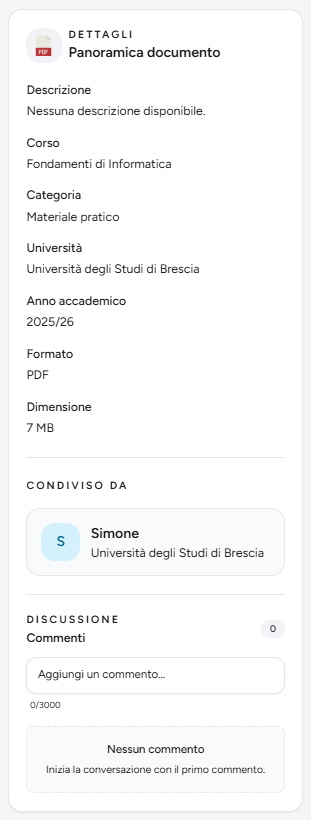
\includegraphics[width=0.3\textwidth]{figures/fig-riprogettazione-fisica/visualizzazione-documento/visualizzazione_documento_1.png}
    \caption{}
    \label{fig:visualizzazione-documento-1}
  \end{figure}

  \item \textbf{Infinite List} (Tidwell): Il pattern descrive la gestione di elenchi di dati tramite uno scorrimento che mantiene l'utente all'interno dello stesso contesto visivo, spesso preferito alla paginazione tradizionale per non interrompere il flusso dell'attività. È stato associato questo approccio alla \textit{Progressive Disclosure}, che consiste nel mostrare inizialmente solo le informazioni essenziali (come i primi commenti) e svelare il resto solo su richiesta dell'utente per evitare il "sovraccarico cognitivo".  

  Problemi di usabilità risolti:
  \begin{itemize}
    \item P79 (I commenti non sono paginati e rallentano la pagina): È stata implementata una visualizzazione progressiva (mostrando ad esempio "5 commenti di 6") con un tasto "Mostra altro". Al superamento dei 10 commenti, l'area diventa scorrevole internamente tramite uno scroll dedicato, evitando che la pagina si allunghi eccessivamente e diventi lenta nel caricamento.
  \end{itemize}

  \begin{figure}[H]
    \centering
    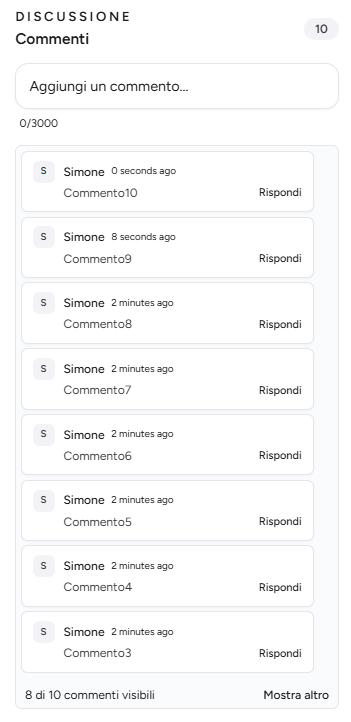
\includegraphics[width=0.3\textwidth]{figures/fig-riprogettazione-fisica/visualizzazione-documento/commenti.png}
    \caption{}
    \label{fig:commenti}
  \end{figure}

\end{itemize}

\paragraph{Altre modifiche}
Sono state apportate correzioni puntuali per migliorare la coerenza del sistema e la sicurezza della community. Sono stati rimossi i feedback visivi ingannevoli che suggerivano interattività dove non presente e sono stati uniformati i testi dei pulsanti per garantire che il linguaggio dell'interfaccia rifletta sempre l'azione che l'utente sta per compiere. È stato inoltre migliorato il sistema di gestione dei file scaricati e introdotto un controllo preventivo sui contenuti per garantire un ambiente di studio adeguato. \\  

Problemi di usabilità risolti:
\begin{itemize}
\item P34 (La voce ”Corso” non è cliccabile): La riga è stata trasformata in semplice testo informativo all'interno della descrizione del documento, eliminando il falso link che creava confusione.
\item P55 (Inconsistenza terminologica ”Scarica” vs ”download”): Il termine è stato uniformato in ”Scarica” sia nella visualizzazione a lista che nel dettaglio del documento, rispettando il principio di coerenza linguistica.
\item P62 (Impossibile segnalare un commento o documento inappropriato): È stata implementata una blacklist di parole non adeguate che impedisce l'invio di commenti offensivi alla radice, proteggendo la community; si tratta di una misura di primo livello, non esaustiva, che intercetta i casi più evidenti.
\item P64 (Il file scaricato ha un nome casuale): Ora il file viene salvato utilizzando il titolo inserito dall'utente durante il caricamento, rendendo il materiale facilmente riconoscibile sul dispositivo dopo il download.
\end{itemize}  

\begin{figure}[H]
  \centering
  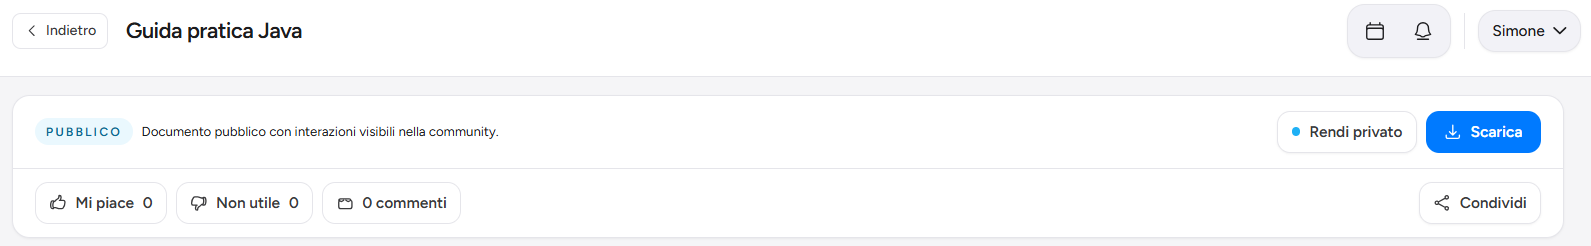
\includegraphics[width=0.8\textwidth]{figures/fig-riprogettazione-fisica/visualizzazione-documento/visualizzazione_documento_2.png}
  \caption{}
  \label{fig:visualizzazione-documento-2}
\end{figure}
  \subsubsection{Generatore trascrizioni e Generatore audio}

\begin{scenario}{Scenario: Trascrizione di appunti audio tramite Sbobinatore AI}
  Ho deciso di provare lo strumento chiamato \textit{«Sbobinatore AI»} su
  BrainBox per convertire la registrazione audio di una lezione in testo. Già dal nome, in realtà, \textbf{non mi è del tutto chiara l'esatta funzione dello strumento} e cosa farà di preciso, ma decido comunque di procedere. Accedo alla sezione dedicata con l'obiettivo di caricare il mio file e lasciare che l'intelligenza artificiale esegua la trascrizione.

  Osservando la pagina vuota, cerco d'istinto un pulsante di caricamento al centro dello schermo. Noto una scritta che dice \textit{«Inizia caricando il tuo primo file!»}, ma \textbf{non avendo l'aspetto di un pulsante cliccabile}, la ignoro. Solo dopo aver guardato meglio la pagina, mi accorgo che il pulsante per creare una nuova trascrizione si trova in alto, nella barra di intestazione: una \textbf{posizione poco
  intuitiva} rispetto a dove stavo guardando.

  Una volta cliccato il pulsante, si apre la schermata per il caricamento. Mi viene chiesto di inserire diverse informazioni.
  Mentre mi preparo a caricare il file, mi rendo conto che \textbf{non è specificato da nessuna parte} quali siano i formati audio accettati né se ci sia un limite di grandezza per il documento. Compilo il campo obbligatorio per il nome e avvio l'operazione.

  A questo punto, il caricamento fallisce e compare un \textbf{messaggio di errore in lingua inglese}. L'avviso è \textbf{molto generico} e non mi spiega il motivo del problema: non so se ho sbagliato il formato o se il file era troppo grande. Questo mi lascia incerto su come rimediare all'errore, oltre a risultare fuori posto in una pagina che finora era tutta in italiano.

  Risolto il problema per tentativi, riesco finalmente ad avviare l'elaborazione. Tuttavia, noto che \textbf{lo strumento non fornisce alcuna indicazione chiara} su come stia procedendo il lavoro. Senza un \textbf{indicatore visivo di avanzamento} o una stima del tempo necessario, resto ad attendere senza sapere se il sistema stia
  effettivamente lavorando o se si sia bloccato.

  Quando il testo finalmente compare, noto che la trascrizione si presenta come \textbf{un unico e lungo blocco di testo}, senza alcuna suddivisione in paragrafi o pause che ne facilitino la lettura.

  Infine, scopro che \textbf{non c'è un comando per salvare il testo} direttamente tra i miei appunti sulla piattaforma: per poterlo conservare e correggere, devo prima scaricare il documento sul mio
  computer, apportare le modifiche e poi ricaricare il file manualmente nella sezione principale dei miei appunti.
\end{scenario}

Lo scenario di utilizzo dello Sbobinatore AI ha evidenziato alcune delle criticità più significative dell'intera applicazione. L'utente si trovava davanti a una pagina dedicata con un nome poco chiaro, pulsanti di avvio in posizioni non intuitive, nessuna indicazione sui formati accettati o sui limiti di dimensione, messaggi di errore in inglese e generici, nessun feedback visivo durante l'elaborazione, output non strutturato e, soprattutto, nessuna possibilità di salvare il risultato direttamente tra i propri appunti senza dover scaricare, modificare e ricaricare 
manualmente il file. Quest'ultima criticità rappresentava il problema di usabilità più grave dell'intera sezione, in quanto interrompeva completamente il flusso di lavoro dell'utente e vanificava l'utilità pratica dello strumento.

La scelta progettuale più rilevante adottata per risolvere questi problemi è stata quella di eliminare le pagine dedicate agli strumenti AI e di integrare le funzionalità di generazione direttamente nella sezione \textit{Appunti}. Questa decisione ha permesso di risolvere in modo strutturale il problema del salvataggio: i file generati, trascrizioni e audio note, vengono ora creati e archiviati direttamente nella sezione \textit{Appunti}, dove l'utente può organizzarli insieme agli altri materiali di studio, allegarli agli esami e gestirli liberamente senza passaggi intermedi. Centralizzare tutto in un unico spazio ha inoltre eliminato la frammentazione tra sezioni separate che rendeva difficile orientarsi 
nell'applicazione.

\paragraph{Design pattern applicati}
\begin{itemize}
\item \textbf{Input Hints} (Tidwell): Il pattern suggerisce di fornire spiegazioni, vincoli o suggerimenti contestuali vicino ai campi di input per prevenire errori prima che accadano. Questo è fondamentale per gestire le aspettative dell'utente riguardo a limiti tecnologici o formati supportati. Nella versione precedente lo strumento non indicava i formati audio accettati né gli eventuali limiti di dimensione, costringendo l'utente a procedere per tentativi; nella versione riprogettata questi vincoli sono resi espliciti direttamente nel primo step di caricamento.

Problemi di usabilità risolti:
\begin{itemize}
  \item P70 (Mancanza di spiegazione sui limiti tecnologici): Nel primo step del caricamento sono stati esplicitati i formati audio supportati e, tramite un'avvertenza dedicata, è stato chiarito che gli strumenti AI possono commettere errori di precisione.
\end{itemize}

\begin{figure}[H]
    \centering
    \begin{subfigure}[b]{0.47\textwidth}
        \centering
        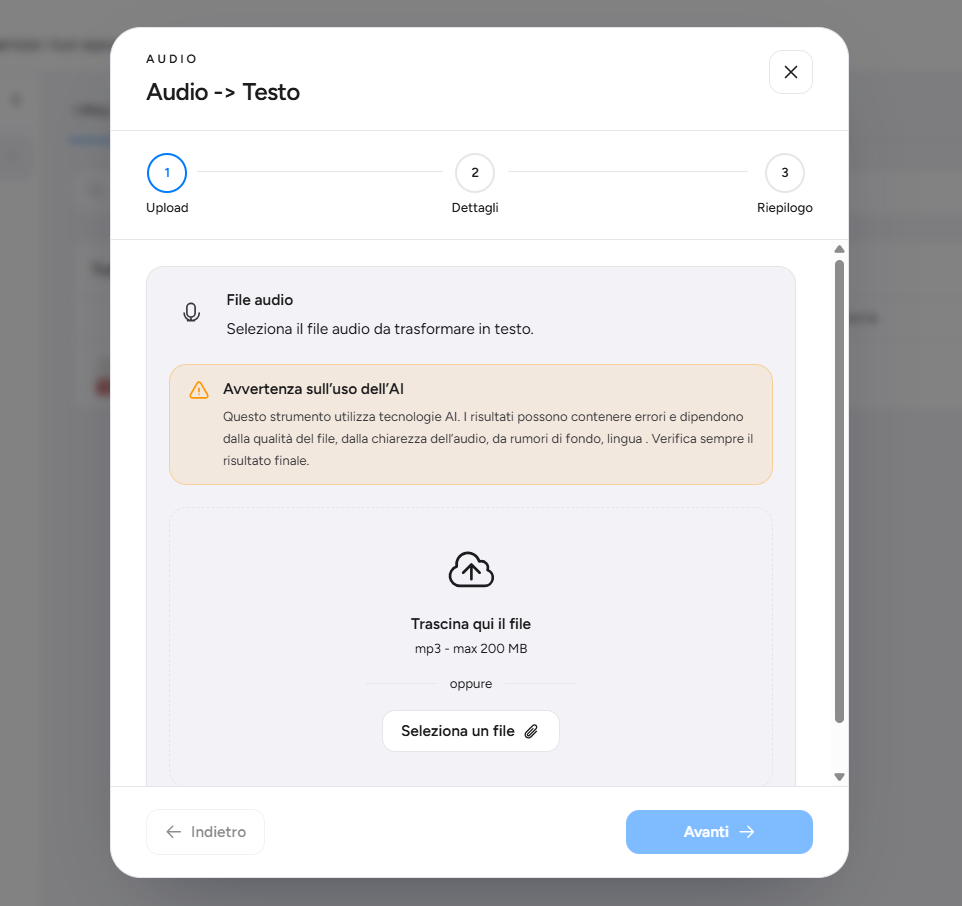
\includegraphics[width=\textwidth]{figures/fig-riprogettazione-fisica/strumenti-ai/ai_1.png}
        \caption{}
        \label{fig:ai_1}
    \end{subfigure}
    \qquad
    \begin{subfigure}[b]{0.47\textwidth}
        \centering
        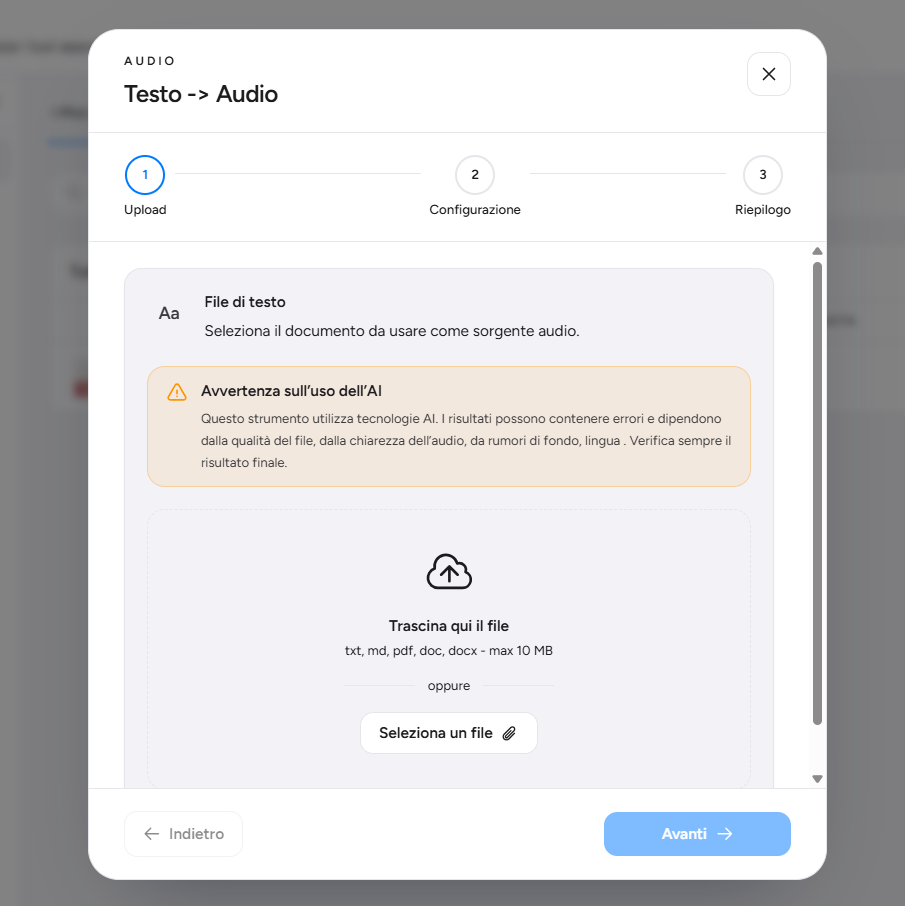
\includegraphics[width=\textwidth]{figures/fig-riprogettazione-fisica/strumenti-ai/ai_2.png}
        \caption{}
        \label{fig:ai_2}
    \end{subfigure}

    \caption{}
    \label{fig:steps1_ai}
\end{figure}

\item \textbf{Spinners and Loading Indicators} (Tidwell): Il pattern prevede di mostrare un'animazione o un indicatore dopo che l'utente ha avviato un'operazione e prima che ci sia una risposta, per comunicare che il sistema sta elaborando e prevenire che l'utente abbandoni il task o pensi che qualcosa sia andato storto. 
  È considerato obbligatorio quando un'operazione richiede più di un secondo, poiché oltre questa soglia l'utente tende a ritenere che l'interfaccia non stia funzionando. 
  Nella versione precedente lo strumento non forniva alcuna indicazione visiva sull'avanzamento della generazione, lasciando l'utente in attesa senza sapere se il sistema stesse effettivamente elaborando. Nella versione riprogettata, invece di un indicatore bloccante mostrato durante l'attesa, la lista file espone in modo persistente lo stato della generazione tramite etichette dinamiche, \textit{In coda}, \textit{In elaborazione}, \textit{Pronto} o \textit{Errore}, permettendo all'utente di monitorare l'avanzamento senza interrompere il proprio flusso di lavoro.

Problemi di usabilità risolti:
\begin{itemize}
  \item P50 (Feedback non chiaro sullo stato di avanzamento durante la generazione): Lo stato di elaborazione è ora sempre visibile nella lista file tramite etichette dinamiche che si aggiornano in tempo reale.
\end{itemize}

  \begin{figure}[H]
    \centering
    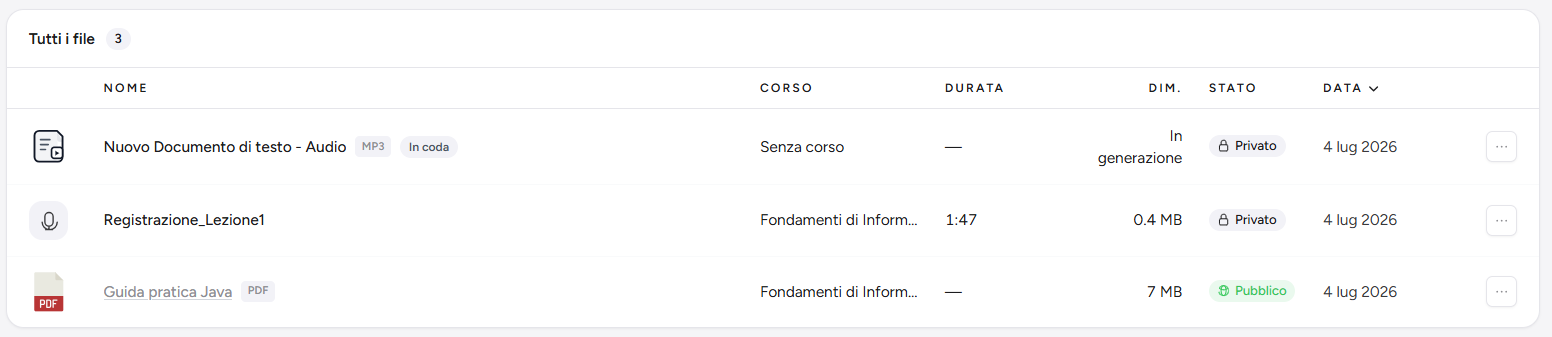
\includegraphics[width=0.8\textwidth]{figures/fig-riprogettazione-fisica/strumenti-ai/ai_4.png}
    \caption{}
    \label{fig:ai_4}
  \end{figure}

\end{itemize}

\paragraph{Altre modifiche}
La struttura delle funzionalità AI è stata radicalmente semplificata eliminando le pagine dedicate e integrando i generatori direttamente nella sezione \textit{Appunti}. \\

Problemi di usabilità risolti:
\begin{itemize}
  \item P41 e P44 (Icone microfono/cassa non funzionanti): Essendo ora le funzioni incorporate in un form di caricamento, le icone "falso bottone" nei titoli sono state rimosse.
  \item P42 (Posizionamento del bottone ”NUOVA TRASCRIZIONE”): Il comando è stato razionalizzato all'interno del flusso di creazione file in \textit{Appunti}. Stessa soluzione per il bottone "NUOVA AUDIO NOTE".

    \begin{figure}[H]
      \centering
      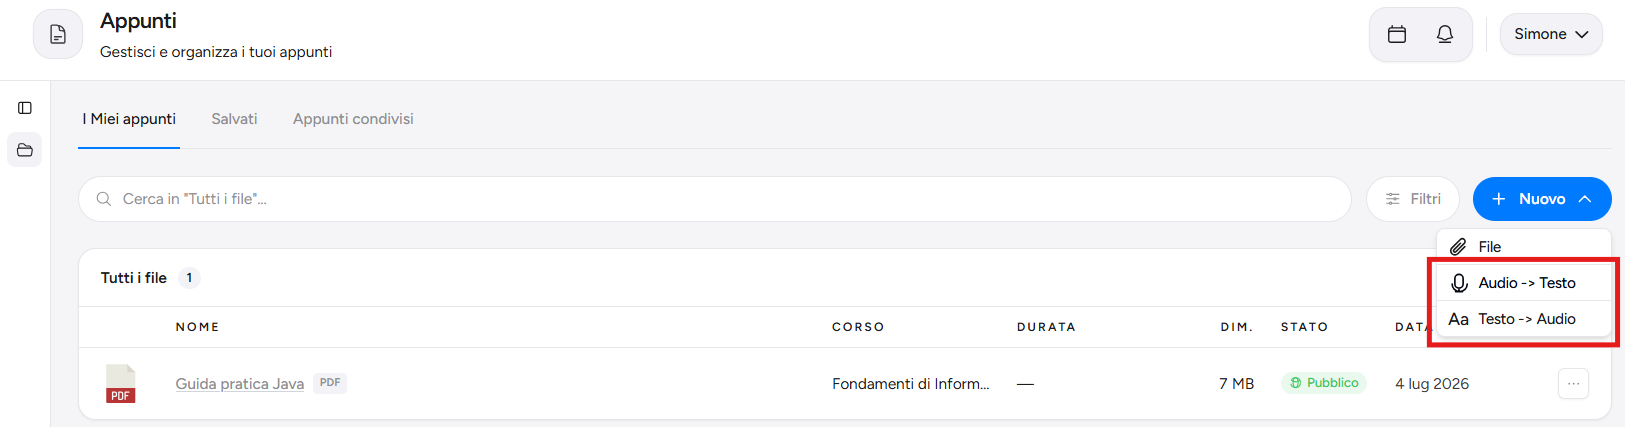
\includegraphics[width=0.8\textwidth]{figures/fig-riprogettazione-fisica/strumenti-ai/ai_3.png}
      \caption{}
      \label{fig:ai_3}
    \end{figure}

  \item P66 (Impossibilità di salvare o allegare): Entrambe le tipologie di file generati (audio e testo) possono ora essere salvate come nuovi appunti e allegate direttamente agli esami.
  \end{itemize}

  Generatore trascrizioni:
  \begin{itemize}
  \item P74 (Mancanza di struttura semantica): Il blocco di testo generato non è più uniforme, ma include ora i \textit{timestamp} per facilitare la consultazione e il riferimento all'audio originale.
\end{itemize}

Generatore audio:
\begin{itemize}
\item P45 (Incoerenza del tasto di conferma): Il pulsante è stato rinominato in \textit{Avvia}, garantendo coerenza terminologica.
\item P67 (Mancanza di supporto iconografico): Gli audio generati sono ora identificati da un'icona specifica nella lista file, permettendo di distinguerli a colpo d'occhio da PDF o altri documenti. Stessa soluzione anche per le trascrizioni.
\end{itemize}

\paragraph{Implementazioni aggiuntive}
La pagina di visualizzazione di una trascrizione è stata completamente riprogettata rispetto alla versione originale, che presentava il testo generato come un unico blocco non strutturato e privo di qualsiasi funzionalità aggiuntiva. Nella versione riprogettata la trascrizione è organizzata in segmenti, ciascuno accompagnato dal relativo intervallo temporale: cliccando su un segmento, il player audio posizionato in fondo alla pagina si sincronizza automaticamente al punto corrispondente dell'audio, permettendo all'utente di navigare rapidamente tra le parti della registrazione. Il contenuto è inoltre suddiviso in due tab, \textit{Trascrizione} e \textit{Riassunto}, così da offrire sia il testo completo sia una versione sintetica del contenuto senza dover scorrere l'intera pagina. In alto è presente un pulsante per scaricare la trascrizione in formato \texttt{.txt}, mentre il pannello laterale destro raccoglie i metadati del file (nome, durata, numero di segmenti, corso e data di caricamento) e un suggerimento contestuale nella parte inferiore. (Figura \ref{fig:ai_5})

  \begin{figure}[H]
    \centering
    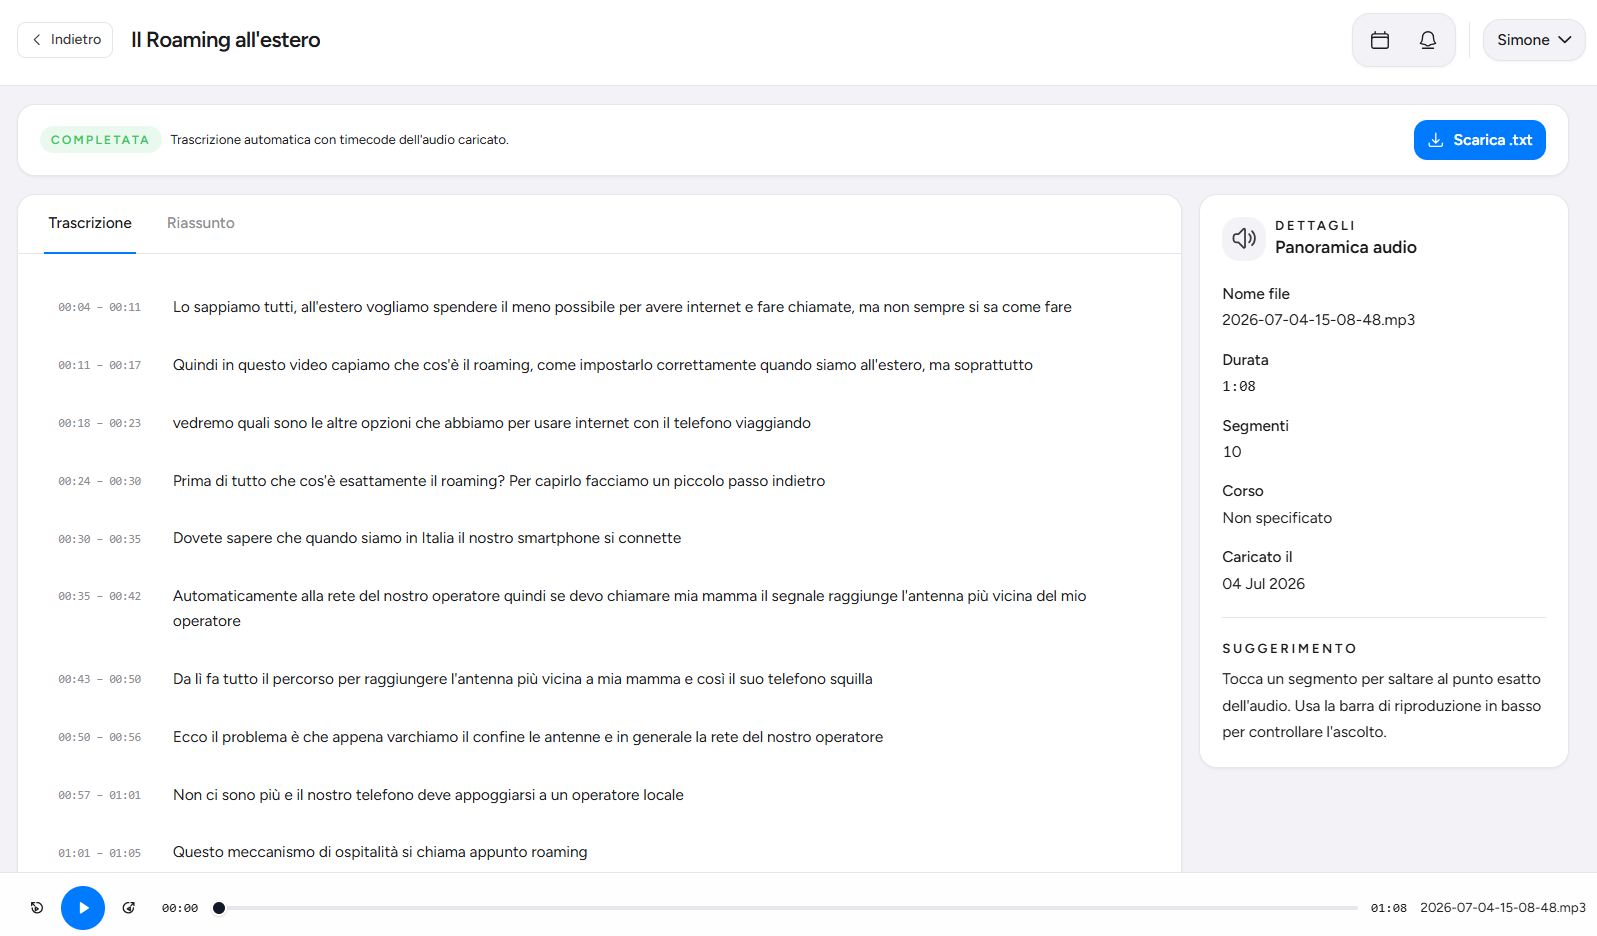
\includegraphics[width=0.8\textwidth]{figures/fig-riprogettazione-fisica/strumenti-ai/ai_5.png}
    \caption{}
    \label{fig:ai_5}
  \end{figure}

Per mantenere coerenza con la pagina di visualizzazione delle trascrizioni, anche la pagina di visualizzazione delle audio note è stata riprogettata adottando la stessa struttura: pulsante per scaricare il file MP3, player audio integrato per riprodurre direttamente il contenuto generato e pannello laterale destro con i metadati del file (nome, data di creazione, durata, tipo, dimensione, formato e voce utilizzata per la sintesi). (Figura \ref{fig:ai_6})

  \begin{figure}[H]
    \centering
    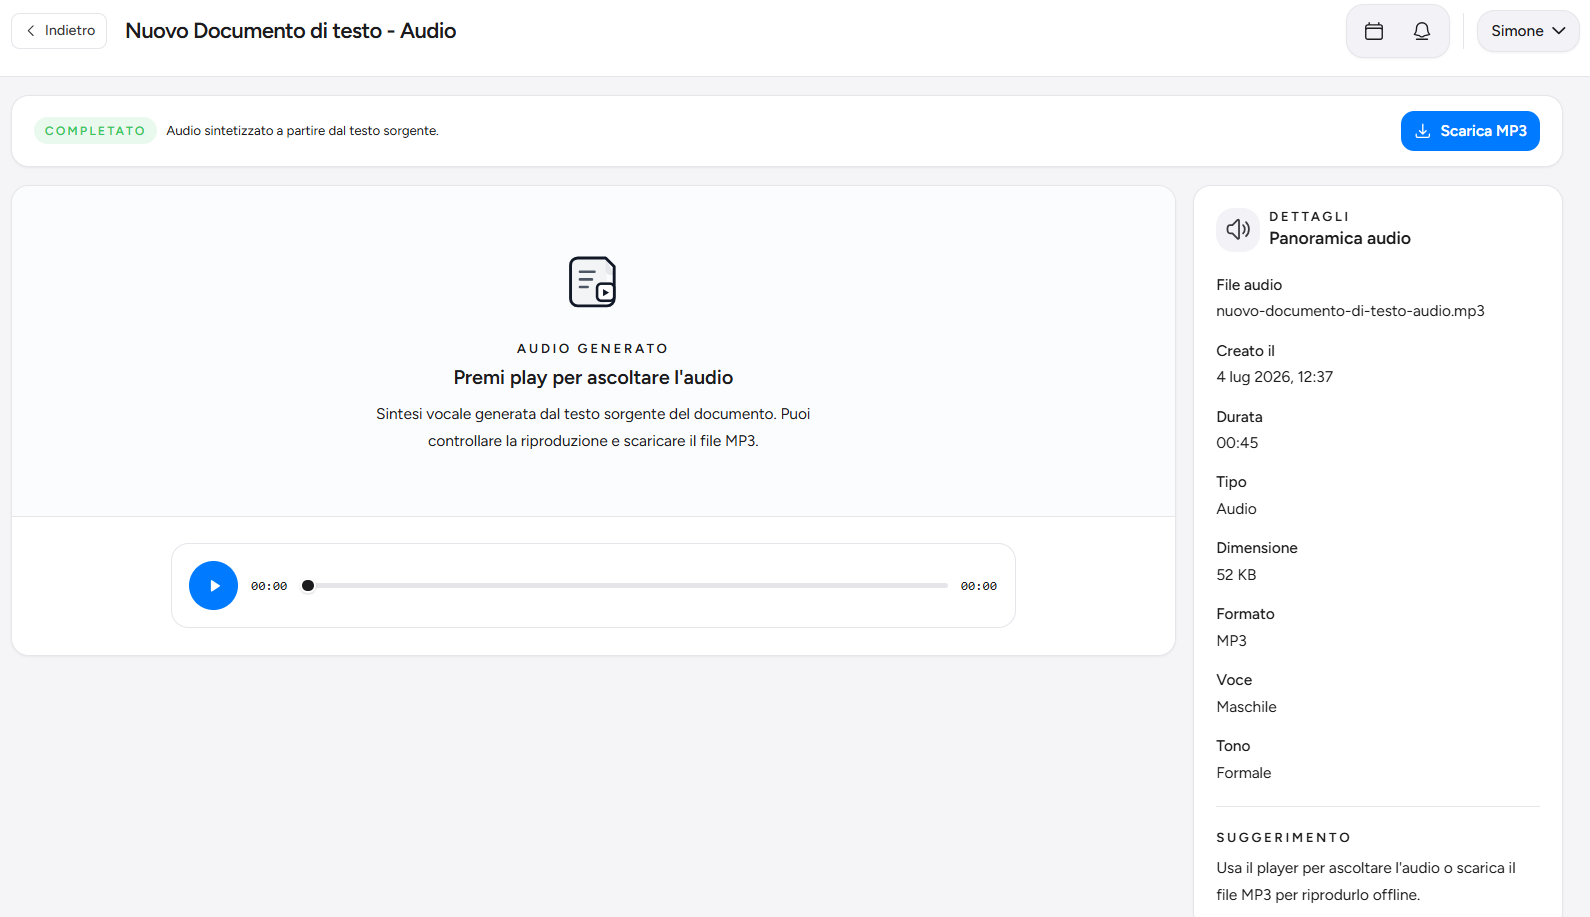
\includegraphics[width=0.8\textwidth]{figures/fig-riprogettazione-fisica/strumenti-ai/ai_6.png}
    \caption{}
    \label{fig:ai_6}
  \end{figure}
\subsubsection{Esami}

\begin{scenario}{Scenario: La pianificazione di un nuovo esame}
  Ho un esame importante tra qualche mese e ho deciso di usare BrainBox per organizzarmi. Inizialmente ho perso diversi minuti a cercare la sezione giusta: non avrei mai immaginato che la pianificazione si trovasse sotto la voce \textit{«StudyFlow AI»}, un nome che trovo \textbf{poco pertinente e fuorviante}.

  Una volta entrato, clicco sul pulsante \textit{«NEW EXAM»}. Il sistema mi chiede di inserire il nome della materia e la data. Dopo aver salvato, l'esame compare in lista e noto che il sistema mi mostra quanti giorni mancano alla prova. Tuttavia, mi rendo conto che \textbf{la configurazione è solo all'inizio}. Per aggiungere i task di studio, non posso farlo durante la creazione, ma devo cliccare in un riquadro separato accanto alla lista; avrei decisamente preferito inserire queste scadenze \textbf{direttamente nel modulo di configurazione iniziale}, non solo in un secondo momento.

  Il percorso diventa ancora più macchinoso quando scopro di poter collegare del materiale salvato ne \textit{«I Miei Appunti»}: anche in questo caso, il sistema \textbf{non me lo ha proposto durante la creazione dell'esame}, obbligandomi a ulteriori passaggi manuali. La cosa più grave, però, accade quando ho bisogno di fare delle modifiche: mi accorgo che \textbf{non esiste un modo per eliminare, rinominare o cambiare la data} di un esame già creato. Se sbaglio, sono costretto a ricominciare da capo.

  Inoltre, se entro nel dettaglio di un esame, mi imbatto in un
  \textbf{calendario non ancora funzionante}. In ogni caso, trovo poco sensato poter accedere ai miei impegni solo quando mi trovo confinato dentro una specifica
  sezione: avrei preferito avere il mio calendario \textbf{sempre a portata di mano},
  da qualsiasi parte del sito. Infine, noto che il sistema crea
  \textbf{confusione tra gli esami passati e quelli ancora da sostenere}, mostrandomi tutto insieme senza alcuna distinzione.
\end{scenario}

Lo scenario mette in luce una serie di criticità che frammentano l'esperienza dell'utente in più punti: dalla difficoltà iniziale nel trovare la sezione, al flusso di creazione incompleto, fino all'assenza di opzioni di modifica e a un calendario non operativo. Il risultato è un percorso discontinuo, in cui l'utente è costretto a tornare più volte sugli stessi passi per completare un'operazione che dovrebbe essere lineare. Per rispondere a questi problemi,
la riprogettazione ha puntato a consolidare l'intero flusso in un'unica esperienza coerente.

Nella versione riprogettata, la sezione Esami, ex \textit{StudyFlow AI}, permette all'utente di gestire i propri esami universitari in un unico spazio: è possibile creare un esame, collegare a esso i propri file di studio già caricati in \textit{Appunti} e definire un elenco di attività da completare per prepararsi al meglio. Le scadenze degli esami inseriti 
vengono inoltre riportate automaticamente nel calendario della navbar, così l'utente può verificare in qualsiasi momento quanto manca a ciascun appello senza dover accedere alla sezione dedicata.

\paragraph{Design pattern applicati}
\begin{itemize}

\item \textbf{Modal Panel} (Tidwell): Il pattern prevede l'utilizzo di un pannello sovrapposto alla schermata corrente che blocca temporaneamente l'interazione con il resto dell'interfaccia, concentrando l'attenzione dell'utente su una singola azione focalizzata. È particolarmente adatto per richiedere conferma prima di operazioni distruttive e irreversibili, come l'eliminazione di un elemento, poiché impedisce che l'azione venga eseguita per errore o distrazione. Nella versione precedente l'eliminazione di una task mostrava un messaggio dal testo ambiguo e inaspettato, e non era possibile eliminare un esame. Nella versione riprogettata entrambe le operazioni presentano un Modal Panel dedicato che chiede esplicitamente conferma prima di procedere, rendendo l'azione comprensibile e reversibile fino all'ultimo.

  Problemi di usabilità risolti:
  \begin{itemize}
    \item P87 (Eliminando una task compare un avviso dal testo strano): È stato sostituito con un Modal Panel dal testo chiaro e coerente con il contesto.
    \item P91 (Impossibile eliminare un esame, solo crearne di nuovi): È stata aggiunta la possibilità di eliminare un esame tramite un'azione dedicata, con relativo Modal Panel di conferma.
  \end{itemize}

  \begin{figure}[H]
    \centering
    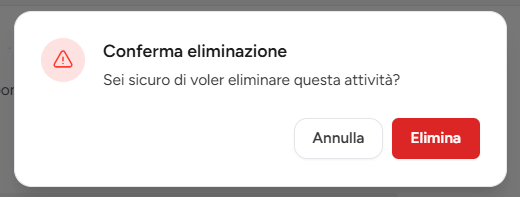
\includegraphics[width=0.6\textwidth]{figures/fig-riprogettazione-fisica/esami/esami_7.png}
    \caption{}
    \label{fig:esami_7}
  \end{figure}

\item \textbf{Error Messages} (Tidwell): Il pattern prevede di mostrare messaggi di errore direttamente accanto al campo che li ha generati, in modo che l'utente capisca immediatamente cosa non va e come correggerlo. Nel form di inserimento di un nuovo esame mancava qualsiasi controllo sulla data: era possibile inserire una 
data antecedente a quella corrente, generando un esame che non veniva poi visualizzato nella pagina principale senza alcuna spiegazione. Nella versione riprogettata, il tentativo di inserire una data passata genera un messaggio di errore direttamente sotto al campo, impedendo il salvataggio e informando l'utente del vincolo violato.

  Problemi di usabilità risolti:
  \begin{itemize}
    \item P84 (Possibile inserire un esame con data antecedente a quella corrente, che poi non viene visualizzato): Il form ora valida la data e genera un messaggio di errore esplicito sotto al campo se si tenta di inserire una data passata.
  \end{itemize}

  \begin{figure}[H]
    \centering
    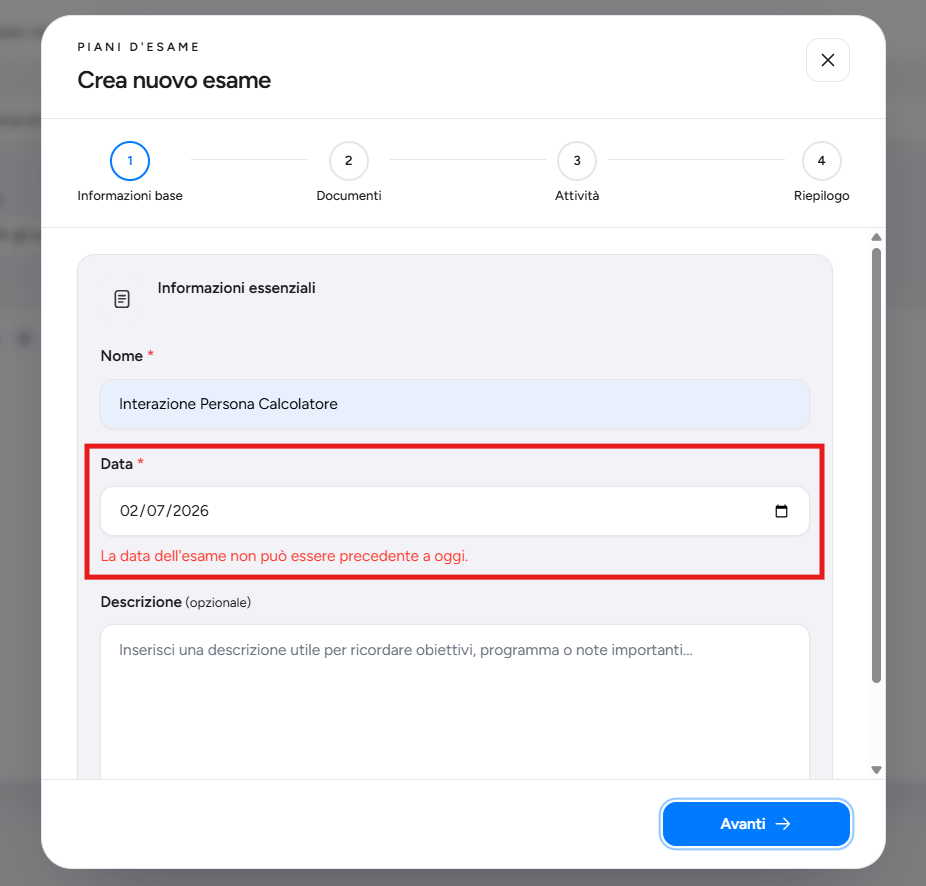
\includegraphics[width=0.6\textwidth]{figures/fig-riprogettazione-fisica/esami/esami_2.png}
    \caption{}
    \label{fig:esami_2}
  \end{figure}

\end{itemize}

\paragraph{Altre modifiche}
È stato adottato un linguaggio coerente con le altre sezioni: la sezione è stata rinominata \textit{Esami} e il pulsante \textit{NEW EXAM} è stato sostituito con \textit{+ Nuovo}, in linea con la convenzione adottata nelle altre sezioni.

Nella visualizzazione dei dettagli di un esame, la gestione del collegamento dei materiali è stata corretta: in precedenza il pulsante \textit{"Aggiungi materiale esistente"} mostrava il messaggio \textit{"Tutti i tuoi documenti sono già stati 
collegati!"} anche quando non era ancora stato caricato nessun file, e il pulsante \textit{"Collega materiali"} compariva privo di funzione attiva. Nella versione riprogettata, quando non sono presenti materiali collegati, compare il messaggio \textit{"Nessun materiale collegato. Usa il pulsante «Aggiungi file» per associare 
appunti esistenti."} e il pulsante risulta correttamente attivo e funzionante. 

\begin{figure}[H]
    \centering
    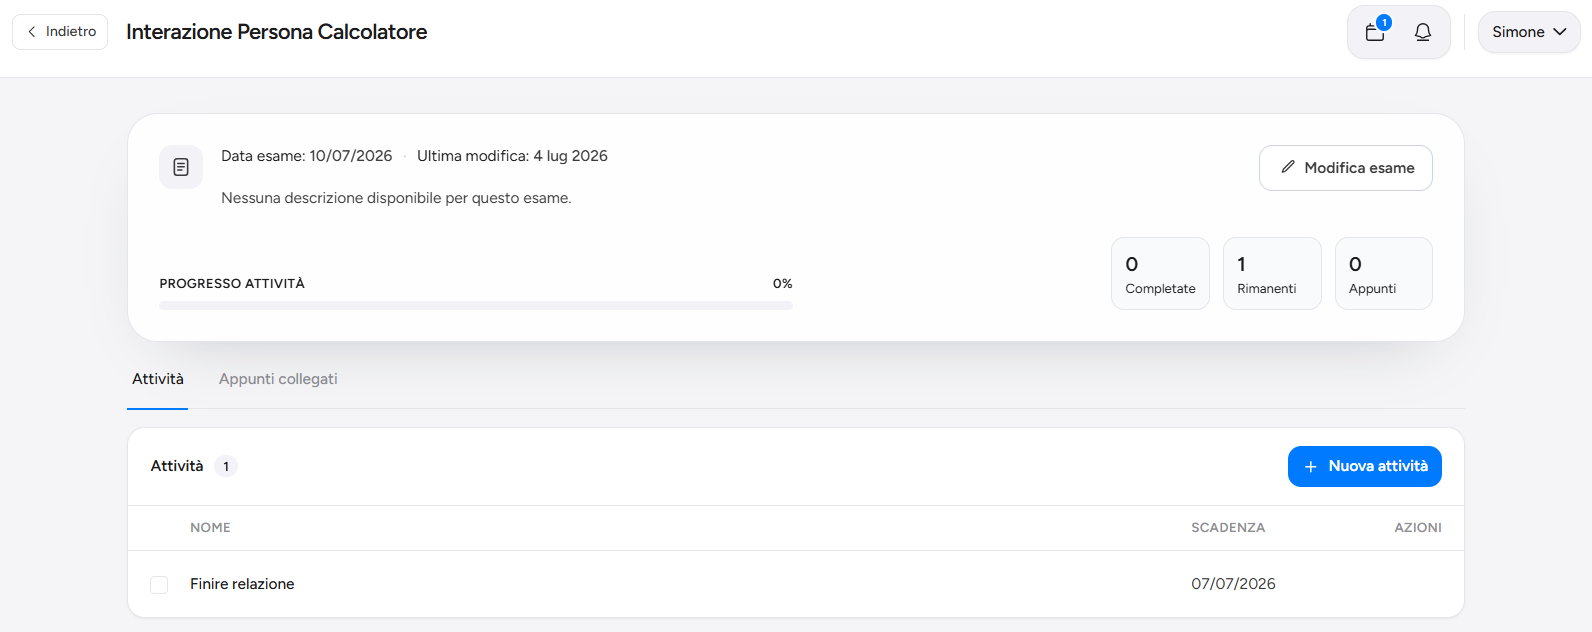
\includegraphics[width=0.8\textwidth]{figures/fig-riprogettazione-fisica/esami/esami_6.png}
    \caption{}
    \label{fig:esami_6}
\end{figure}

Problemi di usabilità risolti:
\begin{itemize}
  \item P46 (Il titolo della pagina non corrisponde al tab selezionato): Il tab \textit{StudyFlow AI} è stato rinominato \textit{Esami} e di conseguenza anche il titolo della pagina.
  \item P47 (Il bottone "NEW EXAM" si trova in una posizione poco funzionale): Il layout è stato allineato a quello delle altre sezioni, con il pulsante \textit{"+ Nuovo"} posizionato in alto a destra accanto alla barra di ricerca e ai filtri.
  \item P48 (Il bottone "NEW EXAM" è scritto in maiuscolo a differenza degli altri): Il pulsante è stato rinominato \textit{+ Nuovo}, in linea con la convenzione adottata nelle altre sezioni.
  \item P49 (La pagina presenta contenuti in inglese): Tutto il testo è stato tradotto in italiano.
  \item P85 (Messaggio "Tutti i tuoi documenti sono già stati collegati!" mostrato anche quando il repository è vuoto): Il messaggio è stato sostituito con un invito contestuale che guida l'utente verso l'azione corretta.
  \item P86 (Il pulsante "Collega materiali" compare senza funzione attiva quando non ci sono materiali): Il pulsante è ora correttamente attivo e funzionante in tutte le condizioni.
\end{itemize}

\paragraph{Implementazioni aggiuntive}
Una delle principali funzionalità aggiunte in questa sezione è quella dei filtri, pensata per aiutare l'utente a orientarsi tra gli esami salvati, risultando particolarmente utile quando questi iniziano ad accumularsi. Si tratta di una funzionalità non direttamente collegata ai problemi emersi durante la valutazione euristica, ma ritenuta fondamentale per migliorare l'esperienza d'uso e per rendere la sezione coerente con quanto già presente in \textit{Appunti} e \textit{Community}.

Il primo è un filtro per stato, che permette di visualizzare tutti gli esami oppure solo quelli preferiti, in corso, completati o scaduti. 
Il secondo è un ordinamento, che consente di riorganizzare la lista per scadenza, nome, progresso o tempo rimanente, in ordine crescente o decrescente.

\begin{figure}[H]
  \centering
  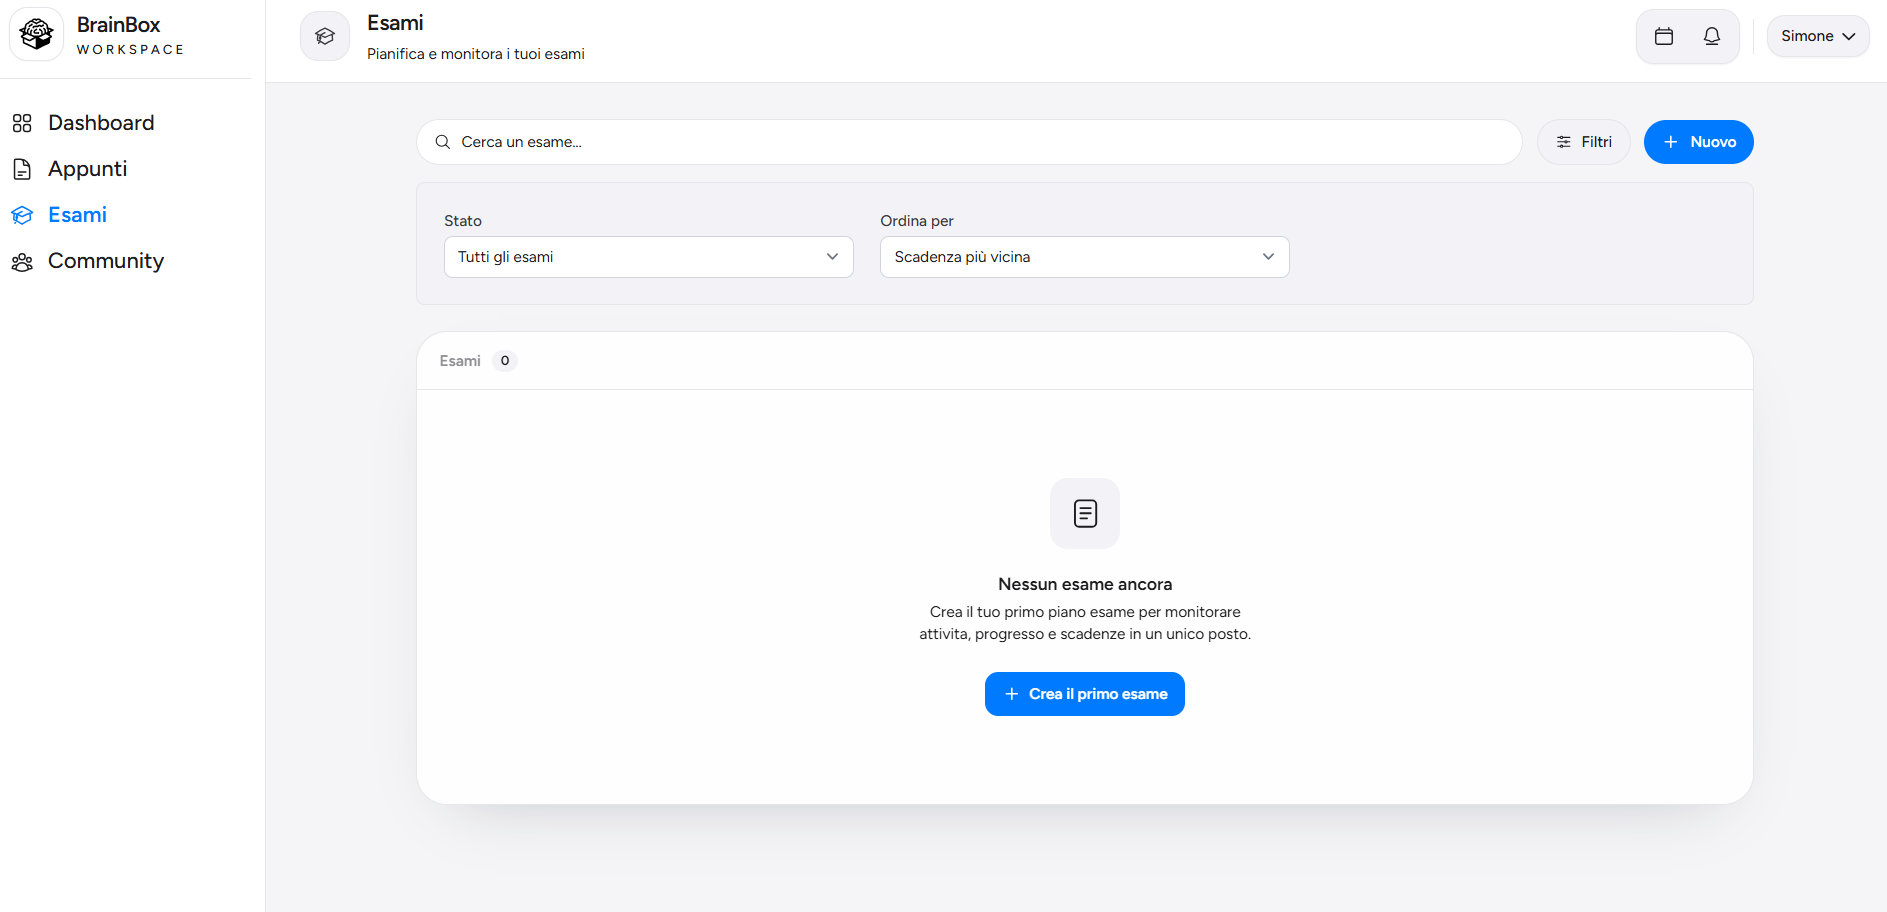
\includegraphics[width=0.8\textwidth]{figures/fig-riprogettazione-fisica/esami/esami_1.png}
  \caption{Pagina iniziale vuota della sezione Esami}
  \label{fig:esami_1}
\end{figure}

\begin{figure}[H]
  \centering
  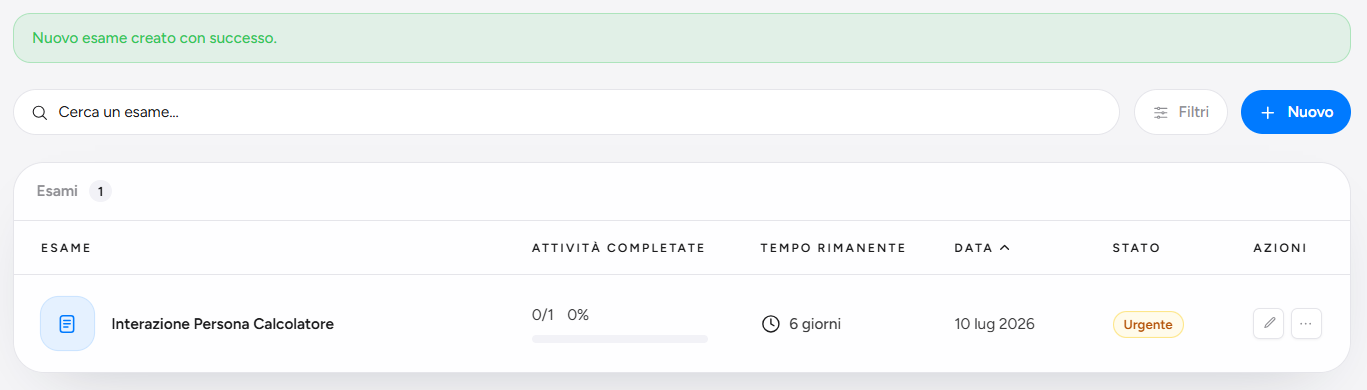
\includegraphics[width=0.8\textwidth]{figures/fig-riprogettazione-fisica/esami/esami_5.png}
  \caption{Pagina iniziale della sezione Esami}
  \label{fig:esami_5}
\end{figure}

Un'ulteriore e fondamentale implementazione ha riguardato l'ottimizzazione del flusso di creazione di un esame. Prima di procedere allo sviluppo dell'interfaccia, si è ritenuto essenziale definire la nuova sequenza operativa attraverso un'analisi dei compiti come riportato in Figura \ref{fig:ta-pianificazione-esame}.

\begin{figure}[H]
  \centering
  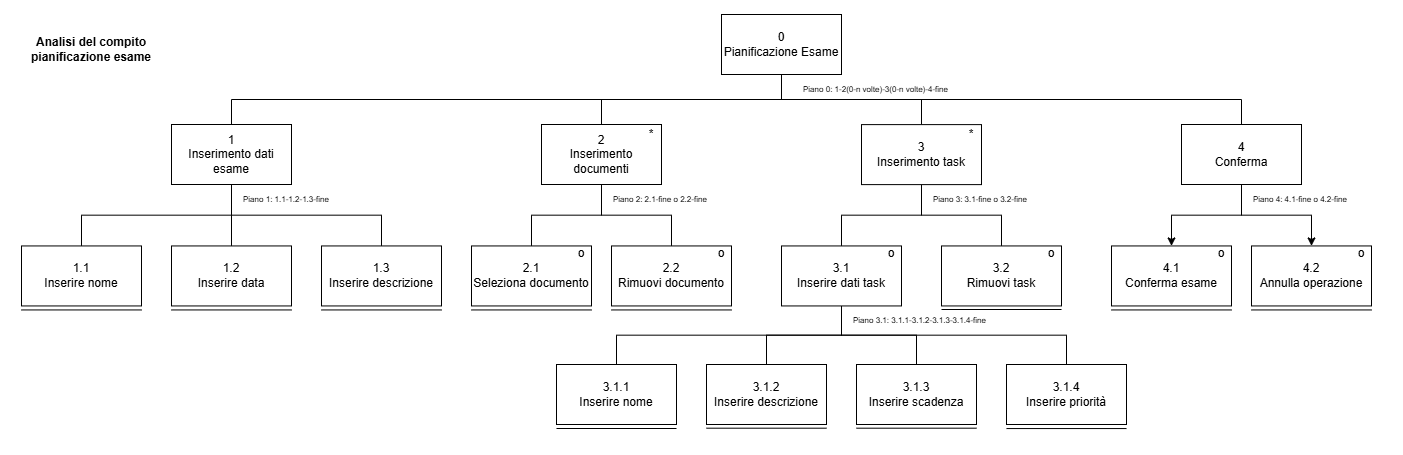
\includegraphics[width=1\textwidth]{figures/fig-riprogettazione-fisica/esami/TA - pianificazione esame.png}
  \caption{Analisi del compito \textit{Pianificazione esame}}
  \label{fig:ta-pianificazione-esame}
\end{figure}

Traducendo concretamente lo schema nell'interfaccia utente, la modale iniziale è stata ampliata introducendo due step aggiuntivi: la definizione delle attività di studio (task) (Figura \ref{fig:esami_3}) e il collegamento dei materiali precedentemente caricati nella sezione \textit{Appunti} (Figura \ref{fig:esami_4}). Questa modifica consente all'utente di configurare un esame completo in un'unica operazione lineare. Al contrario, la versione originale imponeva un processo fortemente frammentato: l'utente era costretto a inserire prima nome e scadenza, per poi doversi spostare in un'area esterna per la creazione dei task e, solo in un secondo momento, accedere al dettaglio dell'esame per collegare i materiali di studio.

\begin{figure}[H]
    \centering
    \begin{subfigure}[b]{0.47\textwidth}
        \centering
        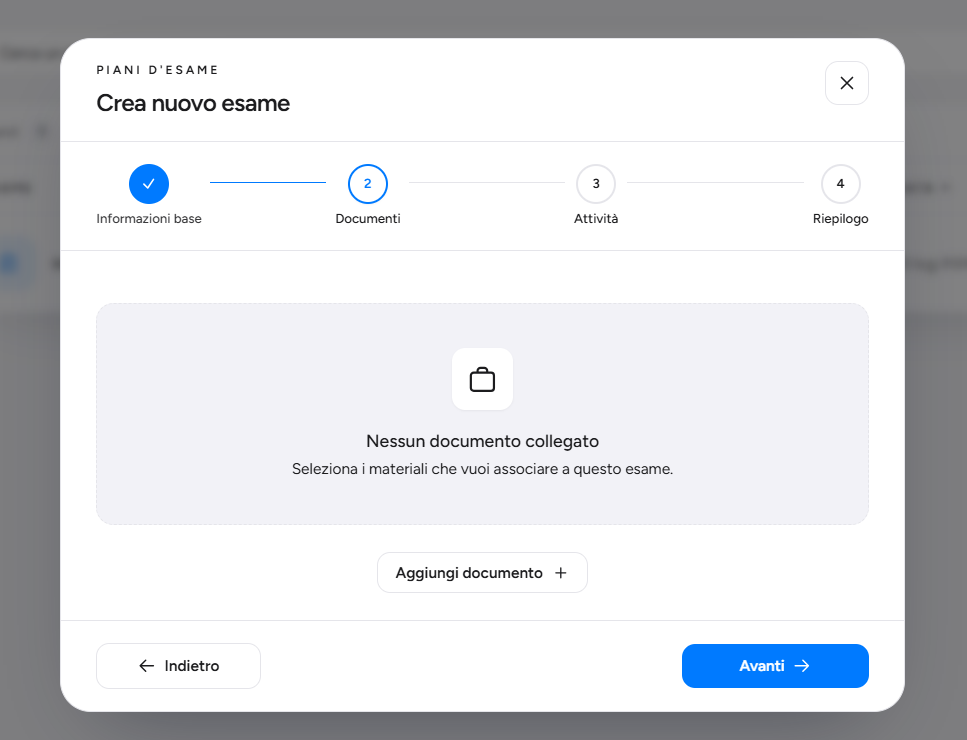
\includegraphics[width=\textwidth]{figures/fig-riprogettazione-fisica/esami/esami_4}
        \caption{Step 2}
        \label{fig:esami_4}
    \end{subfigure}
    \qquad
    \begin{subfigure}[b]{0.47\textwidth}
        \centering
        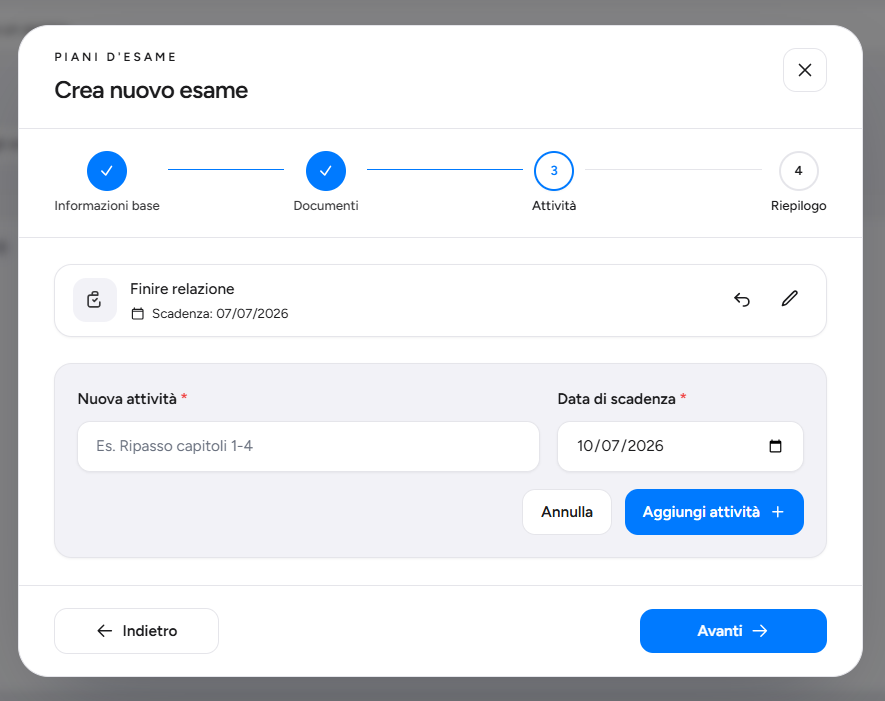
\includegraphics[width=\textwidth]{figures/fig-riprogettazione-fisica/esami/esami_3}
        \caption{Step 3}
        \label{fig:esami_3}
    \end{subfigure}

    \caption{}
    \label{fig:esami_steps}
\end{figure}
\subsubsection{Community}
La sezione Community corrisponde alla ex "Esplora Appunti" della versione
precedente, rinominata per comunicare più chiaramente la sua funzione di spazio condiviso tra utenti. Il layout adottato è il medesimo della sezione "Appunti", scelta che ha permesso di mantenere coerenza visiva tra le due sezioni e di applicare in parallelo alcune delle stesse modifiche: la rimozione della vista a griglia in favore della sola vista a lista, la barra di ricerca per titolo affiancata dai filtri per
metadati e la ridefinizione delle colonne di visualizzazione dei file. Le modifiche specifiche alla sezione Community riguardano invece la gestione della distinzione tra contenuti propri e altrui e la scelta di non introdurre strumenti di organizzazione personale come le cartelle, per mantenere una separazione netta rispetto allo spazio personale già offerto da "Appunti".

\paragraph{Modifiche progettuali}
La visualizzazione a griglia è stata rimossa in favore della sola vista a lista, in quanto risultava inadatta alla consultazione di grandi quantità di file: con decine o centinaia di documenti, la griglia mostra meno informazioni per elemento, presenta inconsistenze visive tra le due modalità e causa problemi di interazione. La vista a lista permette invece di esporre più metadati per ciascun file in modo uniforme, facilitando la scansione e il confronto rapido tra i risultati. \\

Problemi di usabilità risolti:
\begin{itemize}
  \item P36 (Cliccando sull'icona del documento non succede nulla, bisogna cliccare il bordo della card): Con la rimozione della vista a griglia il problema non è più riproducibile.
  \item P37 (In vista griglia mancano data di caricamento e università): La vista a lista espone uniformemente tutti i metadati per ciascun file.
  \item P38 (Il pulsante "Scarica" cambia aspetto tra vista lista e vista griglia): Con la rimozione della vista a griglia il problema non è più riproducibile.
  \item P39 (Il nome dell'autore cambia aspetto tra vista lista e vista griglia): Con la rimozione della vista a griglia il problema non è più riproducibile.
\end{itemize}

\begin{figure}[H]
  \centering
  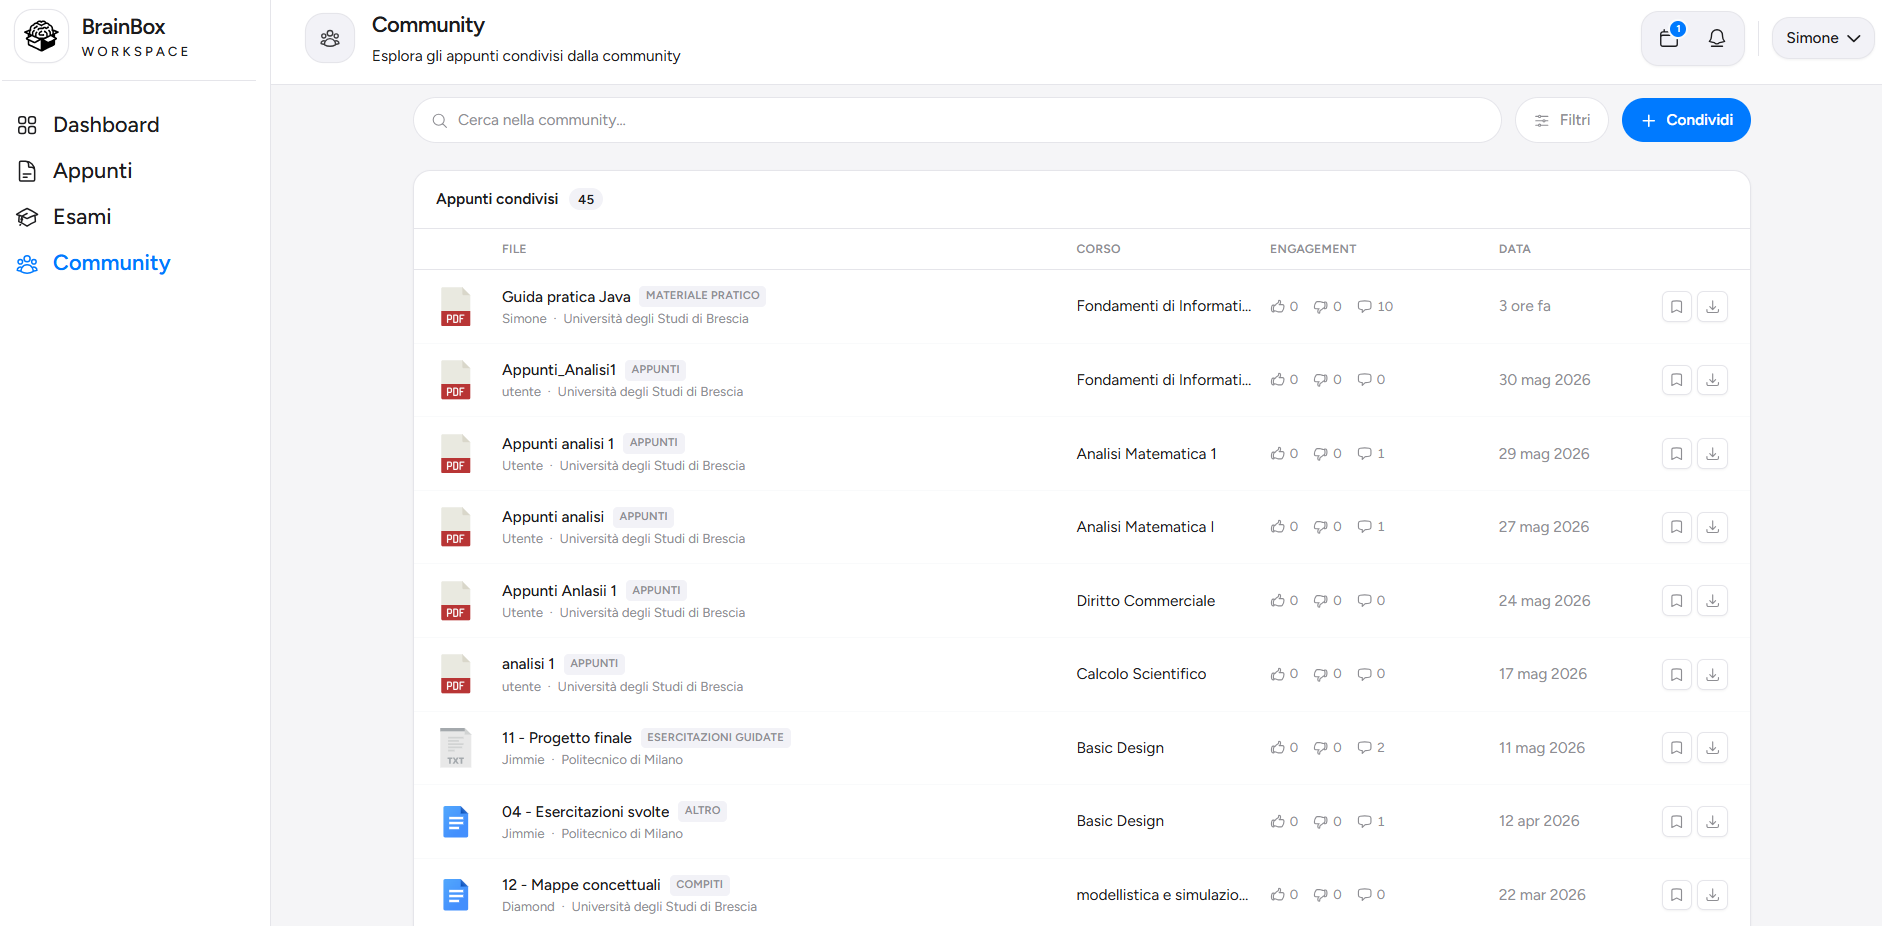
\includegraphics[width=0.8\textwidth]{figures/fig-riprogettazione-fisica/community/community_1.png}
  \caption{Vista a lista sezione Community}
  \label{fig:community_1}
\end{figure}

La barra di ricerca è stata mantenuta per la ricerca per titolo e sono stati aggiunti o corretti i filtri dedicati per i principali metadati, "Università", "Corso", "Categoria" e "Anno Accademico", per permettere all'utente di restringere i risultati lungo dimensioni multiple senza dover digitare query complesse. In questo modo l'utente può combinare liberamente ricerca testuale e filtri per individuare rapidamente i contenuti di interesse. \\

Problemi di usabilità risolti:
\begin{itemize}
  \item P52 (La ricerca è limitata al solo titolo del documento): Sono stati aggiunti o corretti i filtri per i principali metadati, ampliando le possibilità di ricerca.
  \item P57 (Nessun controllo sull'ordinamento e sul filtraggio delle liste): I filtri permettono all'utente di restringere i risultati secondo le dimensioni più rilevanti.
\end{itemize}

\begin{figure}[H]
  \centering
  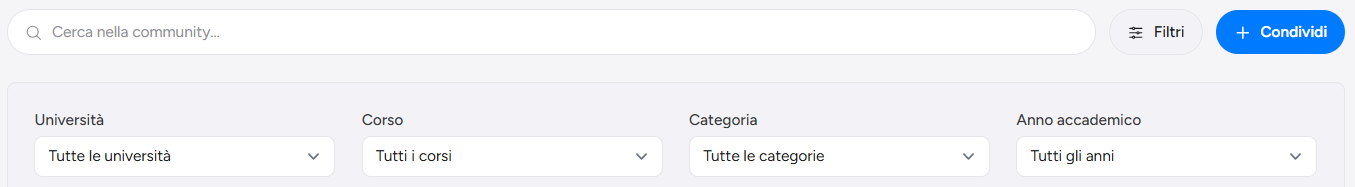
\includegraphics[width=0.8\textwidth]{figures/fig-riprogettazione-fisica/community/community_2.png}
  \caption{Filtri di ricerca della Community}
  \label{fig:community_2}
\end{figure}

La distinzione tra i propri contenuti condivisi e quelli degli altri utenti è stata risolta a livello strutturale tramite i tab della sezione Community. La vista predefinita mostra tutti i documenti condivisi sulla piattaforma, mentre selezionando il tab "Appunti condivisi" viene applicato un prefiltro che mostra esclusivamente i documenti
pubblicati dall'utente stesso. \\

Problemi di usabilità risolti:
\begin{itemize}
  \item P69 (Nessuna distinzione visiva tra proprie risorse e risorse altrui): La distinzione è gestita tramite il tab "Appunti condivisi" che applica un prefiltro sui soli documenti pubblicati dall'utente, senza necessità di distinguerli visivamente all'interno della lista generale.
\end{itemize}

\begin{figure}[H]
  \centering
  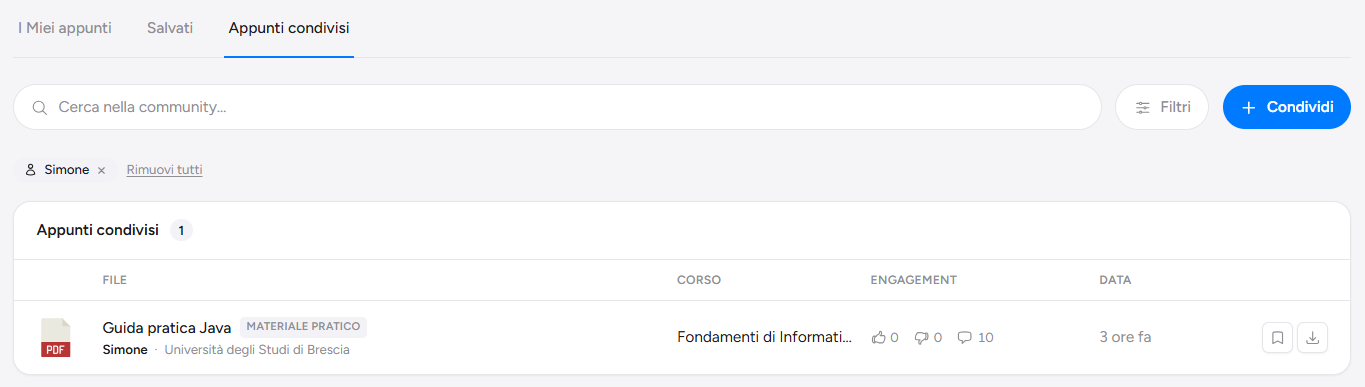
\includegraphics[width=0.8\textwidth]{figures/fig-riprogettazione-fisica/community/community_3.png}
  \caption{Tab "Appunti Condivisi"}
  \label{fig:community_3}
\end{figure}

È stato introdotto un feedback visivo per distinguere i file già visualizzati
da quelli non ancora consultati. \\

Problemi di usabilità risolti:
\begin{itemize}
  \item P61 (Nessun feedback visivo sui file già visualizzati): È stata introdotta una distinzione visiva tra file già aperti e file non ancora consultati: i primi vengono visualizzati con opacità ridotta, in modo che i contenuti nuovi risaltino immediatamente all'interno della lista. La modifica è stata applicata in modo coerente anche nella sezione "Appunti".
\end{itemize}
